%===================================================================================================
%  Chapter : 微分と積分
%  説明    : 微分積分の考え方と計算方法を確認する.
%===================================================================================================
%   %==========================================================================
%   %  Section : 極限
%   %==========================================================================
        \section{極限}
%       %----------------------------------------------------------------------
%       %  Input
%       %    File Name : PhysNote_Math_DifrAndIntg_inf.tex
%       %    説明      : 極限値:限りなく近づけるとは?
%       %----------------------------------------------------------------------
        %   %==========================================================================
%   %  Section : 極限
%   %==========================================================================
        %==================================================================
        %  SubSection
        %==================================================================
            \subsection{数列とは}

        %==================================================================
        %  SubSection
        %==================================================================
            \subsection{等差数列}

        %==================================================================
        %  SubSection
        %==================================================================
            \subsection{等比数列}

        %==================================================================
        %  SubSection
        %==================================================================
            \subsection{等比級数}

        %==================================================================
        %  SubSection
        %==================================================================
            \subsection{無限等比級数}

        %==================================================================
        %  SubSection
        %==================================================================
            \subsection{数列の極限\;\;--「限りなく0に近づける」とは --}
                微分の定義で,$\Delta x$ を「0に近づける」という表現を用いる.
                しかし,この“近づける”という表現は,どうにも,曖昧である.“
                近づける”とはいうものの,その近づける方法がよく分からないし,
                また,どの程度まで近づけられるかもはっきりとしない.そもそも,
                「近づけられるのか」という不安もある.そこで,ここでは“近づけ
                る”という作業とはどのようにすべきかを考える.まず,具体例で考
                えよう.例として,0の“次に”大きい数を考えてみよう.
                自然数で考えるならば,これは1である.しかし,
                今考えているのは,実数の範囲だから,1ではありえない.それでは
                ,0.1か.いや,もっと小さい数の0.01がある.いやいや,0.001,
                0.0001,といくらでも考えられる.この問いには,具体的に数を提示
                して,解答することはできない.それでは,「0の次に大きい数」は
                存在しないのか.0よりも少しでも大きい数は存在するが,“0の次”
                となると,答えられなくなってしまう.この問い自体が,無意味な問
                いだからである.では,なぜこのようなことを考えたかといえば,0
                の次に大きい数を考えるときに,その答えとなる数として,1,0.1,
                0.01,$\cdots$ と0にだんだんと“近づいて”いったからである.「
                近づける」という作業をしたのだ.これを,文字を用いて表現できれ
                ば,「近づける」ということを,もっと納得の行く形で受け入れるこ
                とができよう.今の手順を,もう一度詳しく,考え直そう.最初に,
                0に近い数として,1を考えた.今回は,1を考えたが,実際は0.5でも
                ,0.3でも,その他の数でも,よかった.とりあえず,考察に先立っ
                て,基準となる数を挙げただけである.そして次に最初に挙げた数よ
                りも,より小さい数を考えた.今回は1に対して0.1を挙げたが,最初
                に挙げた数の0よりも近い値であれば,どのような数でもよい.そして
                ,さらに0に近い値,もっと0に近い値へと徐々に0に近づけていった.
                この作業は無制限に続き,終わりがないが,これを自動的に行わせる
                ように,文字で表現できれば,目標を達成できる.今の例とその解答
                手順を,もう少し一般的に扱うために,文字で表現してみよう.0に近
                い数として最初に挙げる数を $a_{0}$ としよう.そして,0と $a_{0}$ の
                値との差 $\mid a_{0}-0 \mid$ を考え,これよりもさらに小さい数が
                存在するとき,そのような数を $a_{1}(<\mid a_{0}-0 \mid)$ とおこ
                う.これを繰り返すと,$a_{0}$,$a_{1}$,$a_{2}$,$a_{3}$,のよう
                な数列が得られる.この数列を $\{ a_{n} \}$ と表現すれば,$n$ が
                大きくなるに伴い,数列 $\{ a_{n} \}$ は0に近づいていくと言える.
                あとは,この作業を式で表現することを考えるのみだ.自然数 $n$ が
                大きくなるということは,「ある任意の自然数 $n_{0}$ に対して,$n>n_{0}$ と
                なるような自然数 $n$ が存在する」
                ということである.例えば,任意の自然数を,$n_{0}=100$ としてみよ
                う.この100に対して,大きい自然数は例えば200がある.そうなれば,
                $n_{0}=200$ と書き換えて,これより大きい数500を考えられる
                .さらに $n_{0}=500$ と書き換えて,$\cdots$ のように考えていけば,
                いくらでも大きな自然数を得ることができる.そして,$n$ の増加に伴
                い,$a_{n}$ と0との差が小さくなるので,その差を $\varepsilon (>0)$ と
                表現すれば,目標とする式表現として,次のように書ける.
                \\
                    \begin{itembox}[l]{限りなく0に近づける}
                        任意の正の数 $\varepsilon$ に対して,自然数 $n_{0}$ を決めることができ,
                            \begin{align}
                                n>n_{0} \quad\Rightarrow\quad \mid a_{n}-0 \mid <\varepsilon
                            \end{align}
                        が成立するならば,数列 $a_{n}$ は0に限りなく近づくと言える.
                    \end{itembox}
                    \\

                このとき,これをもっと読みやすく簡略化した式として,
                    \begin{align}
                        \lim_{n\rightarrow \infty } \{ a_{n} \} = 0
                    \end{align}
                と表現する.

                今回挙げた例の,この $\varepsilon$ に対応するのが,1である.
                この1対応して $n_{0}=1$ と決まる.そして,$n_{0}=1$ に対して,
                これより大きい自然数 $n=2$ を与えることができる.$n=2$ とした
                ときに,$\mid a_{2}-0 \mid < 1$ となるような数 $a_{2}$ が存在
                すれば,$\varepsilon$ として[1より小さい値]が存在するとして,
                $\varepsilon$ がその値で書き換えられる.今回の例では0.1である.
                また,$n_{0}=2$ とも書き換えられる.これで一巡したが,同様に,
                $n_{0}=2$ のとき,これよりも大きい自然数 $n=3$ を与えることが
                でき,$\mid a_{2}-0 \mid < 0.1$ となるような数が存在すれば,
                $\varepsilon$ をその数に書き換える.今回の例では0.01である.
                そして,$n_{0}=3$ とも書き換える.$n_{0}=3$ に対して $n=4$ が
                存在し,$\cdots$ 以下同様.

                このような作業を無制限に続けることができるとき,
                0に近づけることができるということであり,
                また,「限りなく0に近づける」という行為でもある.
                そして,この式によって,「限りなく0に近づける」
                という行為が,いわば“自動的”に行
                .「近づける」という行動を起こさなくても,極限を
                定義することができた.
                    \begin{figure}[hbt]
                        \begin{center}
                            \includegraphicsdefault{suretu_kyokugen1.pdf}
                            \caption{数列の極限}
                            \label{fig:suretu_kyokugen1}
                        \end{center}
                    \end{figure}

                また,上の例では0に近づけるということを考えたが,
                任意の実数に近づけるという作業も
                同じように考えられる.その場合,近づけたい数を $\alpha$ とするならば,
                次のように表現を拡張できる.
                    \\
                    \begin{itembox}[l]{限りなく実数 $\alpha $ に近づける}
                        任意の正の数 $\varepsilon$ に対して,自然数 $n_{0}$ を決めることができ,
                            \begin{align}
                                n>n_{0} \quad \Rightarrow \quad
                                \mid a_{n}-\alpha  \mid < \varepsilon
                            \end{align}
                        が成立するならば,数列 $a_{n}$ は $\alpha$ に限りなく近づくと言える.
                    \end{itembox}
                    \\

                このとき,これをもっと読みやすく簡略化した式として,
                    \begin{align}
                        \lim_{n\rightarrow \infty } \{ a_{n} \} = \alpha
                    \end{align}
                と表現する.


                見ての通り,先ほどの式の0を $\alpha$ で置き換えただけである.
                ちなみに,このような $\alpha $ が存在するとき,
                数列 $\{a_{n}\}$ は $\alpha$ に \textbf{収束} するという.
                また,$\alpha$ のことを数列 $\{ a_{n}\}$ の \textbf{極限} という.
                感覚的にいってしまえば,数列の項の番号 $n$ が大きくなるともなっ
                て,項の値が極限値に近づくということである.

                    \begin{figure}[hbt]
                        \begin{center}
                            \includegraphicsdefault{suretu_kyokugen2.pdf}
                           \caption{数列の極限2}
                           \label{fig:suretu_kyokugen2}
                        \end{center}
                    \end{figure}

                最初に $\varepsilon$ を設定するのは,自然数 $n_{0}$ を必ず決定できる
                ようにするためである.自然数 $n_{0}$ を決定したとしても,$\varepsilon$ は
                全く定まらない.先に $\varepsilon$ を決定しておけば,その範囲に含まれる
                自然数があるはずであり,この内のどれかが $n_{0}$ であるとして,極限の定
                義ができる.

                    \begin{figure}[hbt]
                        \begin{center}
                            \includegraphicsdefault{suretu_kyokugen3.pdf}
                            \caption{数列の極限3}
                            \label{fig:suretu_kyokugen3}
                        \end{center}
                    \end{figure}


                この定義の最大の利点は,複数の数列の極限値に関する,
                加減乗除の定理を証明できる点にある.
                例えば,2つの数列 $\{ a_{n} \}$ と $\{ b_{n} \}$ が
                あるとき,次のような数列を作ってみよう.
                    \begin{align*}
                        \{ a_{n}+b_{n} \} =
                            a_{1}+b_{1}\,,\,\,a_{2}+b_{2}\,,
                            \,\,a_{3}+b_{3}\,,
                            \,\,\cdots\,,
                            \,\,a_{n}+b_{n}\,,\,\,\cdots
                    \end{align*}
                この数列の極限はどうなるだろうか.
                これは簡単で,2つの数列 $\{ a_{n} \}$ と $\{ b_{n} \}$ の極限がそれぞれ,
                    \begin{align*}
                        \lim_{n\rightarrow \infty } \{ a_{n} \}
                            &= \alpha\, \\
                        \lim_{n \rightarrow \infty } \{ b_{n} \}
                            &= \beta
                    \end{align*}
                であるとき,数列 $\{ a_{n}+b_{n} \}$ の極限は,
                    \begin{align*}
                        \lim_{n\rightarrow \infty } \{ a_{n}+b_{n} \}
                        &= \lim_{n\rightarrow \infty } \{ a_{n} \}
                        +  \lim_{n\rightarrow \infty } \{ b_{n} \} \\
                        &= \alpha + \beta
                    \end{align*}
                となる.これを証明するには,「近づける」という表現で極限を説明し
                ただけでは論理的に不可能である.極限を式で定義することで,この定
                義に基づいて,上の公式を証明することが可能になる.


            %==================================================================
            %  SubSection
            %==================================================================
                \subsection{関数の極限\;\;-- $\varepsilon $\,-\,$\delta$ 論法 --}
                数列の極限を考えたついでに,関数の極限も考える.
                考える関数の性質として,全ての点で連続で,全ての点で微分可能な関数を考える.
                関数が連続であるとは,関数に切れ目がないことである.微分可能であるというのは,
                全ての点がなめらかにつながっているということである.

                1変数関数について考える.
                変数 $x$ をもつ関数 $f(x)$ において,ある任意の定点 $x_{0}$ を
                関数 $f(x)$ に代入する.このとき,関数が $f(x_{0})=A$ であったとする.
                つまり,関数 $f(x)$ は,点 $x_{0}$ で,$A$ という値をとると仮定しよう.

                    \begin{figure}[hbt]
                        \begin{center}
                            \includegraphicsdefault{EpDl.pdf}
                            \caption{関数の極限}
                            \label{fig:EpDl}
                        \end{center}
                    \end{figure}

                この場合,関数の極限として,1変数関数 $f(x)$ において,
                   「 変数 $x$ を限りなく $x_{0}$ に近づけると,関数 $f(x)$ の値は,
                    A に近づく.」
                と言える.しかし,これはとても曖昧な表現である.
                数列の極限で考えたときと同じように,
                この「近づける」という行為を,式で表現することにしよう.

                変数 $x$ を定点 $x_{0}$ に近づけると,関数 $f(x_{0})$ は $A$ に近づくが,
                $A$ とは一致しない.つまり,変数 $x$ を定点 $x_{0}$ に近づけているときに
                は, $A$ とは若干異なった値の $A+\varepsilon $ を示す.ここに,$\varepsilon$ は
                任意の正の定数である.$\varepsilon $ のイメージは,とても小さな値をもつ
                定数である.

                さて最初に関数 $f(x)$ に対して,$\varepsilon $ を決めると,
                これに対応して,変数 $x$ の範囲も決まる.その $x$ の範囲を $\delta $ と書こう.
                しかし,この $\delta $ が分かったとき,さらに関数 $f(x)$ が $A$ に
                近づくような範囲 $\varepsilon $ を与えなおすことができる.そうすれば,
                この $\varepsilon $ の変更に伴って,$x$ の範囲 $\delta $ も変わる.そ
                うなれば,変更された $\delta $ に対して,さらに $f(x)$  が $A$ に
                近づくような範囲に $\cdots$.これは無制限に続けることができ,最終的に
                は,関数の極限として,$x$ を $x_{0}$ に近づけたときに,$A$ の値を得る,
                ということになる.

                このように,最初の一回だけ $\varepsilon$ を指定するだけで,
                あとは無制限に自動的に,関数の極限値を得られる.以上をもう
                少し詳しく記述し,式で表現して見よう.

                関数 $f(x)$ において,変数 $x$ を $x_{0}$ に近づけるが,
                $x_{0}$ に一致させないようにするとき,
                $\mid x-x_{0} \mid$ はある正の値 $\delta$ をもつ.
                この $\delta$ のイメージは,$x_{0}$ を
                含むような,変数 $x$ の微小な区間である.
                そして,関数 $f(x)$ には,この微小区間 $\delta$ に対応して,
                $\mid f(x) - A \mid$ という正の値 $\varepsilon$ という値域
                をもつことになる.$f(x_{0})=A$ であるので,$\varepsilon$ が
                より小さくなれば,さらに関数は $A$ からの範囲を狭めていくこ
                とになる.関数 $f(x)$ は連続な関数なので,$\varepsilon$ をさ
                らに小さくすることは可能である.$\varepsilon$ をさらに小さく
                するに伴い,$\delta$ もさらに小さくなっていく.
                もちろん,$\delta$ をいくら小さくしても,その範囲の中には $x_{0}$ が
                含まれている.

                式で書いてみよう.まず,$A$ からのずれの程度の指標である,
                $\varepsilon$ が考えられる.そして,この $\varepsilon$ が
                定まることで,$x$ の範囲もきまり,$\delta$ となるとき,
                    \begin{align}
                        \mid x-x_{0} \mid < \delta \quad
                        \Rightarrow \quad \mid f(x) - A \mid < \varepsilon
                    \end{align}
                であるならば,関数 $f(x)$ は,変数 $x$ を定点 $x_{0}$ に
                近づけたときに,$A$ に収束すると言える.

                今までは連続関数を考えてきたが,実際は,もう少し制限を緩めることができる.
                というのも,関数 $f(x)$ は区間 $I$ のみで連続と定義されていればよく,
                また一方で,$x$ も $x_{0}$ の点で定義されていなくてもかまわない.
                $f(x_{0})$ が定義されていなくても,$x$ は単に $x_{0}$ に近づけるだけ
                であり,一致させるわけではないので,不都合は生じない.

                最初に $\varepsilon$ の存在を確認したのは,このためである.
                もし $\delta$ の存在を先に認めてしまうと,もしかしたら,
                関数が定義されないような範囲を選んでしまう可能性がある.
                そうなれば,上の式は,その関数が定義されていない点に差し掛かったとき,
                極限が存在しないという結論を出してしまう.



%   %==========================================================================
%   %  Section : 積分
%   %==========================================================================
        \section{積分}
%       %----------------------------------------------------------------------
%       %  Input
%       %    File Name : PhysNote_Math_DifrAndIntg_intg.tex
%       %    説明      : 積分学を確認する.
%       %----------------------------------------------------------------------
        %   %==========================================================================
%   %  Section : 積分
%   %==========================================================================
        %==================================================================
        %  SubSection
        %==================================================================
            \subsection{面積は積分によって定義される}
                面積の定義は「縦$\times$横」であるが,この定義は図形ありきのものである.
                しかし,数学的に面積を議論したい場合には,不十分である.面積の数学的
                定義は積分によって定義されるべきである.以下では,積分について考えていこう.
                
                積分を勉強する前に,大事な注意をしておきたい.議論の最初から「面積」という
                言葉を定義なしに使用する.定義なしの「面積」はイメージとして捉えてほしい.
                面積は積分によって定義したいので,積分を定義するのに面積は使ってはいけない
                    \footnote{
                       もし,積分を面積によって定義してしまったら,論理的不整合になる.
                       循環論法になってしまうのだ.
                       積分の定義に面積が必要で,その面積の定義には積分が必要となってしまっては
                       数学的議論が循環してしまう.公理から定義や証明によって演繹的に構築される
                       数学としてこれは絶対に避けるべき.
                    }. 
                そうかと言って,面積のイメージなしに積分を説明するのは困難である.
                では,どうするか.無駄のない論理を構築したい場合は,面積という語彙を使わずに
                単なる計算として積分を定義したあとに,この積分によって面積を説明すべきであろう.
                しかし,これではイメージがしにくく学習効率がわるい.だから,このノートでは
                妥協して,積分の説明に「面積」という語彙を使用する.ただし,積分を定義する前に使用する
                「面積」はあくまでも日常言語的なイメージであり,数学的概念ではない.

                面積の定義をしなくても積分を定義できる.だけど,「面積」のイメージなしに
                積分の定義を理解することは困難である.だから,積分の定義を説明するのに「面積」という
                語彙を使用する.積分が定義できた暁には,それまで使用した「面積」のイメージを
                一切擦れたふりをしよう.積分の定義は単なる計算であり,「面積」の概念は使われていない.
                積分の定義を理解するのに使用する「面積」は補助輪である.積分が理解できたら,補助輪を
                外そう.そして,積分によって補助輪(「面積」)を定義するのだ.

        
        =================================================================
        %  SubSection
        %==================================================================
            \subsection{長方形の面積公式に対する疑問}
                積分は面積と深くかかわりがある.そこで,ここで改めて,
                面積とは何かを考えてみる.

                目標は任意の一変数関数 $f(x)$ の積分を定義することだ.
                以下,変数 $x$ は $f(x)$ の独立変数であり,実数であるとする.

                面積といえば,最
                も基本的な面積公式として,長方形の面積の公式
                    \begin{equation*}
                        \mbox{縦} \times \mbox{横}
                    \end{equation*}
                がある.
                    \begin{figure}[hbt]
                        \begin{center}
                            \includegraphicslarge{ChouhoukeiMenseki.pdf}
                            \caption{長方形の面積}
                            \label{fig:ChouhoukeiMenseki}
                        \end{center}
                    \end{figure}

                長方形の面積というものを,小学校でどのように教わったか忘れてしまったが,
                おそらく,天下り的に教わったのではないかと思う.しかし,強引に押し付けられた
                この式を,単純に鵜呑みにするには少々抵抗がある.
                そこで次節から,改めて長方形の面積はなぜ「縦の長さ$\times$横の長さ」なのかを,
                できるだけ,合理的に説明してみよう.

        %==================================================================
        %  SubSection
        %==================================================================
            \subsection{長さとは何か}
                まず,長さという概念を考えないといけない.これは何も難しく考えることない.
                なぜなら,私たちは定規を使って長さを測るという行為をすでに会得しているから
                である.少し畏まった形で,説明してみよう.

                長さは,数直線状の2点の間の距離として捉えれば良い.
                    \begin{figure}[hbt]
                        \begin{center}
                            \includegraphicsdefault{NagasaToSuuchokusen.pdf}
                            \caption{棒の長さと数直線}
                            \label{fig:NagasaToSuuchokusen}
                        \end{center}
                    \end{figure}

                棒の長さ $l$ を考えるなら,棒を数直線に並べて置いて,棒の両端に
                対応する数直線上の2点 $a$,$b$ ($a<b$ となるように置く)から,
                    \begin{equation*}
                        l = b - a
                    \end{equation*}
                とすれば,長さを数で表せる.

                さらに言えば,棒を置く位置は
                どでもよいから
                    \footnote{
                        棒を置く位置によって,棒の長さが変わることがないという
                        前提の上での話である.
                    },
                棒の一端を数直線上の原点,つまり,数値0に対応するようにして,
                さらに,もう一端を正の数値 $x(>0)$に対応するように置ける.
                    \begin{figure}[hbt]
                        \begin{center}
                            \includegraphicsdefault{NagasaToSuuchokusen_0.pdf}
                            \caption{棒の長さ}
                            \label{fig:NagasaToSuuchokusen_0}
                        \end{center}
                    \end{figure}

                すると,
                    \begin{equation*}
                        l = x - 0 = x
                    \end{equation*}
                となる.$l=x$ となって,数値 $x$ がそのまま棒の長を示すことになる.

                なんだか面倒な言い回しになってしまったが,要は,
                棒の長を測るには,棒の端に定規の0をあてて,
                もう一方の端に対応する数値 $x$ を読めば,
                この数値 $x$ が知りたかった棒の長さ $l$ と
                同一視できるということである.単に,定規を使って
                棒の長さを測るという行為を,式を使って丁寧に説明
                しただけだ.

        %==================================================================
        %  SubSection
        %==================================================================
            \subsection{長方形の面積とは何か}\label{sunsec:ChouhoukeiNoMensekiToha}
                長さは,数直線上の点により表現できることがわかった.では,
                面積はどうだろうか.たしかに,私たちは長さという概念だけで
                はなく,平面的な広がりというものも感じ取ることができる.そ
                して,様々な広がりの大きさを感じてもいる.例えば,土地の広
                さが良い例だ.土地を持っていると,国に税を払わないといけな
                いが,この税の支払い額は所有している土地の広さに大きく影響
                する.当然,広い土地を持っているほど,多額の税金を国に収め
                ないとならない.現実には,土地の面積でけで税の支払い額が決
                まるわけではないが,ここでは,話を単純にするため,面積のみ
                で支払う税金の額が決まるとしよう.つまり,同じ大きさの土地
                を持っている者は,同額の税を払うことになる.こうなると問題
                になるのが,土地の大きさの測り方である.どうやって,土地の
                広さが同じだとか,どちらが小さいとかをきめれば良いのだろう
                か.もし,正確に表すことができなければ,例えば,同じくらい
                の広さの土地を持つものが二人いたとして,支払う税額が両者で
                異なれば,争いが起こることは必至である.幸いにも,この問題
                を解決するすべを,すでに私たちは持っている.面積という概念
                が,その解決の鍵だ.ある決まった広さを基準として,その何倍
                かで広さを表すのである.これにより,広さを数量的に比較する
                ことができるのである
                    \footnote{
                        実際には,面積の測定方法はどうするかといった問題が
                        ある.同じ土地の面積を測るのに,毎回異なる結果を出
                        すような測定方法ではダメだ.かなり深刻な問題だけど
                        ,ここで無視しよう.
                    }.

                長さが数直線状の2点で表すことができたなら,面積も同じように
                考えることができないだろうか.全く同じように考えることはでき
                ないが,この考え方を真似ることはできる.数直線を2つ使うのである.
                    \begin{figure}[hbt]
                        \begin{center}
                            \includegraphicslarge{Menseki00.pdf}
                            \caption{面積}
                            \label{fig:Menseki00}
                        \end{center}
                    \end{figure}

                2つの数直線を用意し
                    \footnote{
                        この2つの数直線の目盛の間隔の長さは,
                        実のところ異なっていてもよいが,ここでは考えやすいように,
                        目盛の間隔は同じであるとしよう.
                    },
                直角に交わるようにする.このような行為を,2つの
                直線を \textbf{直交} させるといい,また,
                この2つの直線は直交しているという.
                考えやすいように,両数直線ともに,原点で直交させよう.

                2つの数直線が直交している部分の近くに,長方形を置く.
                置き方はいろいろ考えられるが,長方形の辺が用意した数直線
                に平行になるようにしよう.すると,各辺の頂点を数直線上の
                数値に対応するようになる.つまり,辺の長さが数によって表現
                できるのである.

                長方形のもつ辺はの数は,縦2本と横2本で,合わせて4つだが,
                縦と横の2本づつの辺の長さは同じである.つまり,
                長方形の形を明確にするには,縦1個と横1個の2つの辺の長さが
                分かれば良い.縦の長さを $m$,横の長さを $l$ とおく.
                縦の長さ $m$ は,辺の頂点が数直線上の $a$,$b$ に対応
                しているとき($a<b$ となるようにする),
                    \begin{equation*}
                        m = b - a
                    \end{equation*}
                である.横方向の長さについても同じように考えて
                ($c<d$ となるようにする),
                    \begin{equation*}
                        l = d - c.
                    \end{equation*}
                長方形の面積はこの2つの長さ $l$,$m$ によって,確定する.
                長方形の面積を表す記号を,$S_{\mbox{\small{長方形}}}$ としたとき,
                $S_{\mbox{\small{長方形}}}$ は $l$ と $m$ を用いて,
                    \begin{equation*}
                        S_{\mbox{\small{長方形}}} = l \times m
                    \end{equation*}
                と定義される.
                これは数直線上の数値 $a$,$b$,$c$,$d$ で表せば,
                    \begin{equation*}
                        S_{\mbox{\small{長方形}}} = l \times m = (d-c) \times (b-a)
                    \end{equation*}
                となり,ひとつの数値に確定する.

                面積とは,2つの独立した数直線上にある,それぞれの区間の長さ $l$,$m$ に
                よって特徴付けられるものである.
                小学校では,「長方形の面積は縦$\times$横である」と
                押し付けられるように教わったが,縦や横とはなんのことかはそれほど明確
                には説明されていなかった.ここでは,縦と横を直交する2つの数直線である
                ように,置き換えることで明確にすることができた.

                しかし,面積は,なぜ,乗算で定義されているのだろうか.加算で定義しても
                よさそうではないか.また,少々おかしいかもしれないが,減算や除算で
                も,論理的に矛盾することのないように,面積を定義することもできるの
                ではないか.もしかしたら,予想通り
                    \footnote{
                        確かめてないからわかりません.もしかしたら,簡単に否定されて
                        しまうかもしれない.
                    },
                乗算以外でも定義可能かもしれない.しかし,広さを数で表すのに最も
                直感と合うものは,掛け算である.例えば,横の長さが1だけ増えるとしても,
                長方形には縦の長さもあるから,その分だけ余計に面積が増える.
                式で書けば,もともと面積が $S_{\mbox{\small{長方形}}}=l\times m$ で
                あった場合に,$l$ が1増えるとで,
                    \begin{equation*}
                        S_{\mbox{\small{長方形}}} = \left( l+1 \right) \times m
                                                  = l \times m + m
                    \end{equation*}
                となって,たとえ $l$ が1しか増えなかっとしても,面積は $m$ だけ
                増えることになるのである.縦横にぎっしりと詰めたタイルを,さらに
                横にその数を増やすときには,縦の枚数分だけのタイルが必要になるの
                である.乗算による定義はこのイメージと一致するのだ.
                    \begin{figure}[hbt]
                        \begin{center}
                            \includegraphicslarge{MensekiToKakezan.pdf}
                            \caption{面積はなぜ掛け算で定義されるか}
                            \label{fig:MensekiToKakezan}
                        \end{center}
                    \end{figure}

            \begin{memo}{一般的な形の面積}
                ちょっと関係ないことになるが,ついでに任意の図形の
                面積について考えてみよう.

                たしか,小学校では,一般的な形の面積を測る方法
                として,基準となる面積が1のタイルを持ってきて,
                その任意の形にを覆うのにひつようなタイルの枚数を
                数える,ということをしたはず.この考え方は,とても
                大切な考え方である.とても素朴で,それこそ,小学生でも
                理解できるのだけど,すごく重要なことを含んでいる.

                もちろん,ここで用意した
                タイルは同じ形のものなので,任意の形をした図形に対して
                ぴったりと覆うことはできず,足りない部分や,はみ出してしまう
                部分も生じる.小学校では,「だいたいこのくらい」で終わってし
                まっただろうが,この考え方をもう一段階進めてみると,任意の形
                をした図形の面積を正確に表現できるようになる.その一段階は
                案外に低い.とても小さいタイルを用意すれば良いのである.
                タイルが小さいほど,隙間を詰めやすくなり,タイルの覆う面積が
                本来の任意の図形の面積に近づく.
                \begin{figure}[hbt]
                    \begin{tabular}{cc}
                        \begin{minipage}{0.5\hsize}
                            \begin{center}
                                \includegraphicsdouble{MensekiToZahyou.pdf}

                                (A)
                            \end{center}
                        \end{minipage}
                        \begin{minipage}{0.5\hsize}
                            \begin{center}
                                \includegraphicsdouble{MensekiToZahyou_dtl.pdf}

                                (B)
                            \end{center}
                        \end{minipage}
                    \end{tabular}
                    \caption{面積}
                \end{figure}


                この考え方は,微分積分学の心に直結する大切な精神を含んでいるので,
                もう一度,繰り返しておこう.直感的に分かりきっていることだけど,
                大変大切な考え方である.

                任意の大きさの長方形を1つ用意して,この1つを複製する.
                用意した長方形の面積は,すでに知っているとする.それで,
                複製した長方形を,面積を知りたい図形の内側に,できる限り稠密
                    \footnote{
                        稠密:隙間なく,ぎっしりと詰まっている様子を,\textbf{稠密} で
                        あるという.ここで使った「できる限り稠密」の意味は,本来の「稠密」の意味
                        からずれているが,隙間の面積が最小になるようにという意味で,「できる限り稠密」
                        という表現を使った.
                    }
                になるように並べる.そして,任意の図形の面積を,並べたすべての長方形の
                面積の合計で近似するのである.もちろん,隙間の文だけの誤差は生じる.
                この誤差が気になるようだったら,はじめに用意する任意の大きさの長方形を
                より小さいものにすれば,それだけ隙間を埋めることができ,その誤差を小さ
                くできる.

                ここで,誤差を「小さく」できると言ってしまった.
                この言い方では,どれだけ誤差を
                小さくできるのかが不明確で,曖昧さを含んでしまう.
                この曖昧さを解消するために厳密には,$\varepsilon - \delta$ 論法を
                使うのであるが,物理学を学ぶ上では,このような厳密さにはそんなにこだわる
                必要はないので,ここでは少々細かいことには目をつぶって,先に話を
                進めていこう
                    \footnote{
                        ただし,もちろん,一度も厳密に考えないというはよくない.
                        暇なときに,物理学を学ぶのに飽きたときに,数学の教科書を
                        読んでおくべきだ.ここで厳密さを無視したのは,あくまでも
                        物理学を行う上では無視しても支障がないからであり,重要で
                        ないからということではない.
                    }.
            \end{memo}

            \begin{memo}{「直角」とは何か}
                2つの直線が「直交する」ということは,
                その2つの直線が直角に交わっていることであると,
                上に記述した.では,「直角」とはなんだろうか.
                交わる角度が $\pi/2$(度数表記では90${}^{\circ}$)で
                ある場合に,直角に交わっていると表現する.
                この説明に従うと,$\pi/2$ は
                円の一周する角度 $2\pi$ の$1/4$ だから,その円の
                2つの直径が円を4等分する角度で交わっている,
                と言うことになる.何が4等分なのかといえば,それは円の
                面積に他ならない.
                    \begin{figure}[hbt]
                        \begin{center}
                            \includegraphicslarge{ChokkakuTohaNanika00.pdf}
                            \caption{円の面積と直交する2つの直線}
                            \label{fig:ChokkakuTohaNanika00}
                        \end{center}
                    \end{figure}

                となると,直角を説明するより先に,面積について説明すべき
                である.しかし,上に説明した考え方に従うと,円の面積を知るには,
                無限に小さな長方形でその円を覆わないとならない.
                そして,ひとつの長方形の面積は,
                上の記述
                    \footnote{
                        \ref{sunsec:ChouhoukeiNoMensekiToha}節参照.
                    }
                によれば,直交する2つの直線という概念を元に,
                説明されるものである.

                さて,語彙の説明の循環に気づいただろうか.直角を説明する前に,面積について
                説明しようとしたのだけど,その面積の説明をするのに,直角という考え方を
                使ってしまったのである.つまり,この説明では,面積と直角の両方の語彙について,
                説明がなされていないということである.

                では,上の説明のどこに間違いがあったのか.答えは簡単だ.「直角に交わる」ということを,
                視覚的な直感に頼ってしまったことである.なぜだか知らないが,人間の目には,「直角」が
                他の角度よりも特別な角度であると,感じてしまう.この感覚が,このような間違いを起こした
                と考えてよいだろう.つまり,より大げさに言うなら,図形の性質の視覚に頼った説明は,
                論理に矛盾を生じやすいということである.

                そうなると,どう正せばよいかということに関心が向かうが,一番手っ取り早い方法が,
                後に説明することになる,\textbf{ベクトルの内積$\cdot$外積} という概念を使うこと
                である.どういう事かといえば,
                「ある条件式
                        \footnote{
                            先走って,書いておくと,2つのベクトル $\ba$,$\bb$ があるとき
                            (ただし,$\ba$,$\bb$ ともに零ベクトルでないとする),
                            $\ba\cdot\bb=0$ であるならば,$\ba$ と $\bb$ は \textbf{直交} していると
                            いう.「ベクトル」という単語を,「直線」と置き換えることで,
                            2つの直線が直交する条件を得ることができる.

                            詳細は,
                            \ref{subsec:VecNaisekiFig}節(\pageref{subsec:VecNaisekiFig}ページ),
                            \ref{subsec:VecNaisekiArg}節(\pageref{subsec:VecNaisekiArg}ページ),
                            \ref{subsec:VecNaisekiStt}節(\pageref{subsec:VecNaisekiStt}ページ),
                            \ref{subsec:VecGaiseki}節(\pageref{subsec:VecGaiseki}ページ)を参照.
                        }
                が成り立つとき,そして,その場合に限り,2つの直線は直交しているという」
                といった,説明になるのだ.

                言いたかったことは,\textbf{上記の説明には,矛盾点が含まれる}ということであり,
                この点に注意してほしい,ということである.直感的に説明しようとしたばっかりに,
                このような矛盾した記述を行ってしまった.
                さらに白状すれば,このノートでは,多かれ少なかれ,この種の矛盾した
                説明を行ってしまうこととなる.しかし,このような矛盾した説明は,
                物理学を直感的に説明しようとする場合には,回避ができないと思われる
                    \footnote{
                        少なくとも,私には,物理学を論理的に矛盾なく説明するだけの力はないし,
                        それがこのノートの目的ではない.このノートの目的の一つは,自然界の現象を
                        物理学を通して,ごく直感的にみることである.
                    }
                なので,このノートを読む場合には,少々矛盾した説明にめをつむっていてもらいたい.
                また,矛盾しているか否か意識しながら,読み進めてもらいたい.
            \end{memo}

        %==================================================================
        %  SubSection
        %==================================================================
            \subsection{関数と,図形の面積}
                長方形の面積について,改めて考え直した.そして,一般の図形の
                面積の求め方の考え方も紹介した.そして,いよいよ,次に積分の
                定義にとりかかるのであるが,いきなり定義を紹介したところで,
                意味不明で消化不良を起こしかねない.なので,少しずつ段階を踏んで,帰納
                的
                    \footnote{
                        帰納的:具体例から一般的に通用する表現を得ることを,
                        「\textbf{帰納的} な手段で,一般規則を得る」などという.
                        学問は,主として,帰納的な考え方によって理論が組み立て
                        られる.なぜなら,世の中には具体例しか存在しないからで
                        ある.具体例の共通点を洗い出して,より一般に通用する規則
                        を見つけるのである.それが数学では公理であったり,物理学で
                        は法則と言われたりするものである.
                    }
                に積分の定義について考える.

                目標は,一般の図形の面積が計算できるようになること,である.
                しかし,いきなり一般の図形を考えることは難しいので
                    \footnote{
                        少なくとも,私にとっては,難しいです.
                    },
                まずは,以下のような状況を考える.一般の図形の面積を
                考えるには,図\ref{fig:IntegFuncKangaeKata00}のように考えると良い.
                    \begin{figure}[hbt]
                        \begin{center}
                            \includegraphicslarge{IntegFuncKangaeKata00.pdf}
                            \caption{$S$ は関数 $f(x)$ と $g(x)$ の間の面積とみなせる}
                            \label{fig:IntegFuncKangaeKata00}
                        \end{center}
                    \end{figure}

                まず,面積を知りたい図形があり,その面積が仮に計算可能であったとして,
                その面積を $S$ としよう.面積 $S$ を知る方法として,まず,図形の縁
                    \footnote{
                        縁:「ふち」と読んでください.「えん」ではありません.
                        図形の周囲を囲む縁のことを言っているんです.
                    }
                に着目する.どうするかというと,この図形の縁を上下に分けて見るのである.
                そして,上方の縁が属する関数 $f(x)$ を仮想的に用意する.
                下方についても同じように,関数 $g(x)$ を用意しよう.図形の縁の上下の端は,
                両方共に,$x_{1}$,$x_{2}$(ただし,$x_{1}<x_{2}$ とする)である.
                そして,次の計算を行う.
                    \begin{enumerate}
                        \item 関数 $f(x)$ と $x$ 軸の間(縦方向)の面積を,
                              $x_{1}$ から $x_{2}$ の間(横方向)で計算し,
                              その値を $S_{f}$ とおく
                        \item 関数 $g(x)$ と $x$ 軸の間(縦方向)の面積を,
                              $x_{1}$ から $x_{2}$ の間(横方向)で計算し,
                              その値を $S_{g}$ とおく
                        \item $S=S_{f}-S_{g}$ により,求めたい面積 $S$ を得る
                    \end{enumerate}


                この方法により,一般的な図形の面積を求めることができる.ただし,
                関数 $f(x)$ や $g(x)$ が存在する場合のみに限られてしまうのだが
                    \footnote{
                        この意味で,「一般的」と言ってしまうのは,少々誇張である.
                    }.

                次節より,このような図形の面積の計算の仕方を学習する.まずは,
                関数 $f(x)$ と $x$ 軸との間の面積を考える.これがわかれば,
                $g(x)$ に対しも全く同じだから,$S=S_{f}-S_{g}$ が計算できるようになる.

                \begin{memo}{一般的な図形の例}
                    上のような考え方ができない図形をひとつ紹介しておこう.
                    図\ref{fig:IntegFuncKangaeKata02}を参照.
                    \begin{figure}[hbt]
                        \begin{center}
                            \includegraphicslarge{IntegFuncKangaeKata02.pdf}
                            \caption{関数 $f(x)$ と $x$ 軸の間の面積}
                            \label{fig:IntegFuncKangaeKata02}
                        \end{center}
                    \end{figure}

                    これでは,図形の縁の上半分の関数 $f(x)$ や下半分の関数 $g(x)$ など,
                    どう考えても作ることはできない.

                    残念ながら,これらの図形の面積をどう扱うかについては,
                    このノートでは考えない.これ以上の深入りはしたくない.
                    物理学で使うのは,関数の作る面積が重要なのであり,
                    一般の図形の面積まで考える必要はない
                        \footnote{
                            もしかしたら,使わなければならないのかもしれないが,
                            今のところは必要としない.ただし,面白い問題であるので,
                            次の教科書を読むことを勧める.

                            (教科書)志賀 浩二 [著] ,
                                        「数学30講シリーズ -- 解析入門30講」,
                                        朝倉書店,1988(初版)
                        }.
                \end{memo}

        %==================================================================
        %  SubSection
        %==================================================================
            \subsection{「関数 $f(x)$ と $x$ 軸の間の面積」とは}
                最終的な目的は,「関数 $f(x)$ と $x$ 軸の間の面積を計算すること」
                である.イメージは図\ref{fig:IntegFunc00}のようなものである.
                    \begin{figure}[hbt]
                        \begin{center}
                            \includegraphicslarge{IntegFunc00.pdf}
                            \caption{関数 $f(x)$ と $x$ 軸の間の面積}
                            \label{fig:IntegFunc00}
                        \end{center}
                    \end{figure}

        %==================================================================
        %  SubSection
        %==================================================================
            \subsection{関数 $f(x)$ に与える条件}
                今までは,何の断りもなしに,「関数 $f(x)$」と書いてきた.しかし,
                実は,これから考える関数 $f(x)$ には,ある条件をみたしている必要
                がある.それは,
                「\textbf{連続} であり,かつ, \textbf{微分可能} である関数」
                というものだ.しかし,ここでは,「連続」だとか「微分可能」だとかの
                専門用語をまだ説明していないので,この条件はとりあえず,考えなくてよい.
                これらの用語については,微分を学習するときに説明する.
                それで,関数 $f(x)$ については,今しばらくの間,一次関数とか二次関数,
                三角関数,指数関数を指しているというように思っていてもらいたい.

        %==================================================================
        %  SubSection
        %==================================================================
            \subsection{変数 $x$ のとりうる値の制限}
                関数 $f(x)$ は,一般的に考えれば,$x$ 軸全体に定義される.しかし,
                これは面積を考える場合には不都合なことである.というのも,$x$ の範囲を指定して
                やらないと,面積を計算できないのである.そこで,この $x$ のとりうる値を
                制限してやって,その制限した区間における $f(x)$ の面積を考えることにする.
                このような考え方で面積を計算する手法のことを,\textbf{定積分} という
                    \footnote{
                        なぜ,わざわざ,「積分」に「定」という文字を付けるのかといえば,
                        あとで,\textbf{不定積分} といわれる計算手法を紹介するからである.
                        不定積分は,微分の逆演算として知られるものだ.後ほど,詳しく説明
                        しよう.
                    }.
                定積分を定義することが,この章の最終的な目標である.

        %==================================================================
        %  SubSection
        %==================================================================
            \subsection{「近似的な面積」という考え方}
                \begin{mycomment}
                    では,積分の定義を説明していこう.とは言っても,
                    一般的に,関数は色々とクネクネしていて,直接的に面積を計算する
                    ことは不可能である.そこで,次のような考え方を使う.近似的な面
                    積の値を計算するのである.
                \end{mycomment}

                近似的な面積を計算方法の説明に入ろう.どうするかというと,まず,
                $x$ 軸をある有限個の区間に区切る.この区間の個数は何個でもいい
                    \footnote{
                        有限個であることを忘れないでね.ちなみに,後で,この個数 $N$ を
                        無限大にもっていきます.無限大に持っていくことで,近似値を真の
                        値にさせることができるんだ.
                    }.
                なので,個数を $N$ 個と
                しよう.この区間の分割は,長さを当分にしなくても良い.
                そうすると,$x$ 軸のそれぞれの区間には,ある長さが各々対応しているはず
                である.なので,それらの長さを,右端から,$\Delta x_{1},\,\Delta x_{2},\,\cdots,\,\Delta x_{N}$ と
                書くことにする.区間の長さが等分であるという条件はないから,一般には
                $\Delta x_{1} \neq \Delta x_{2}$ である
                    \footnote{
                        もちろん,“たまたま長さが同じになってしまいました”という
                        こともある.だけど,長さが同じだろうが異なっていようが,
                        最終的には関係の無いことなので,無視してしまおう.
                    }.

                $x$ 軸を $N$ 個に分割したので,$N$ 個の区間ができたわけだ.この $N$ 個の区間で
                それぞれ,代表点を一つ決める.代表点の決め方には任意である.これらの代表点を
                決めると,その代表点に対する関数の値も定まる.
                代表点を $x_{1},\,x_{2},\,\cdots,\,x_{N}$ と書こう.以下,番号 $i$ を
                使い,$x_{i}$ とまとめて,略記する.
                図\ref{fig:INTEG_LIM00}参照.
                    \begin{figure}[hbt]
                        \begin{center}
                            \includegraphicslarge{INTEG_LIM00.pdf}
                            \caption{区間を $N$ 個に分割}
                            \label{fig:INTEG_LIM00}
                        \end{center}
                    \end{figure}

                第一の区間である $\Delta x_{1}$ の部分に注目しよう.
                この区間をみると,この区間で関数の値が仮に一定値を取るとすれば
                    \footnote{
                        ひとつの区間で関数が一定値をとるなんていう仮定は,
                        強引すぎるかもしれない.しかし,ここは我慢して,先へ読み進めて
                        ほしい.すぐに,この強引さは解消されることと思う.ここでは,あくまでも,
                        面積の近似値をどう考えるかを説明するだけであり,近似するという意味では,
                        そんなに強引な仮定ではないだろう.
                    },
                横 $\Delta x_{1}$,縦 $f(x_{1})$ の長方形が一つ作れる
                    \footnote{
                        以降では,「横の長さ」と記述すべきところを,単に,「横」と記述する.
                        「縦の長さ」についても,単に,「縦」と記述する.煩わしさを無くすため
                        である.単なる縦$\cdot$横いう言葉との区別は文脈で判別できるので,
                        省略した表現をする.
                    }.図\ref{fig:INTEG_LIM01}参照.
                同様に,横 $\Delta x_{2}$,縦 $f(x_{2})$ の長方形も一つ作れる.同じように $N$ 個の
                すべての区間に対して長方形を考えられる.
                それらは,横 $\Delta x_{i}$ と 縦 $f(x_{i})$ の長方形の面積 $\Delta x_{i}f(x_{i})$ である.
                ここで作った長方形の面積を足しあわせて,その値を $S_{N}$ とした場合,
                    \begin{equation*}
                        S_{N} = \sum_{i=1}^{N}\Delta x_{i}f(x_{i})
                                = \Delta x_{1}f(x_{1}) + \Delta x_{2}f(x_{2}) + \cdots + \Delta x_{N}f(x_{N})
                    \end{equation*}
                と計算される.

                なんでこんな長方形を考えて,それらを加え合わせて $S_{N}$ を求めたかというと,
                $S_{N}$ が,今求めるべき「関数 $f(x)$ と $x$ 軸の間の面積」の近似値として,
                使えるからである.図\ref{fig:INTEG_LIM01}参照.
                    \begin{figure}[hbt]
                        \begin{center}
                            \includegraphicslarge{INTEG_LIM01.pdf}
                            \caption{関数 $f(x)$ と $x$ 軸の間の面積}
                            \label{fig:INTEG_LIM01}
                        \end{center}
                    \end{figure}

                \begin{memo}{和の記号 $\sum$}
                    $\sum$ は総和の記号である.“シグマ”と読む.
                    $\displaystyle\sum_{i=1}^{N} f(x_{i})\Delta x_{i}$ は
                    以下の式の略記である.
                    \begin{equation*}
                        \sum_{i=1}^{N} f(x_{i})\Delta x_{i}= f(x_{1})\Delta x_{1}+ f(x_{2})\Delta x_{2}+
                        \cdots +  f(x_{N-1})\Delta x_{N-1}+ f(x_{N})\Delta x_{N}
                    \end{equation*}
                \end{memo}

                \begin{memo}{番号 $i$ を用いた表現(例 $x_{i}$)}
                    番号 $i$ を用いた表現について,説明する.というのも,私がこの表現に
                    つまずいてしまったからである
                        \footnote{
                            私は,この表現の意味を,なかなか理解できなかった.
                            最初は,意味がわからず,式変形を追うことしかできなかった.
                            これを理解するのに,半年以上(1年かも)かかった記憶がある.
                            線形代数(ベクトルと行列を扱う数学の分野)が得意なひとには,
                            なんの苦労もなしに,理解できることなんだけど$\cdots$.
                        }.

                    この表現を導入したい理由は,例えば,上の場合で,
                    この分割した $\Delta x_{1},\,\Delta x_{2},\,\cdots,\,x_{N}$ と,
                    それに対応した代表点 $x_{1},\,x_{2},\,\cdots,\,x_{N}$ の任意の一組を表現することが多くなる
                    から,その略記法を使いたいからである.

                    番号というだけに,$i=1,\,2,\,3,\,\cdots,\,N$ とする.つまり,
                    番号 $i$ は,自然数のうちどれかひとつの数を表すもの,とするのである.この番号 $i$ を
                    用いることで,$x_{1}$ や $x_{2}$ などを,ひっくるめて表現できるのである.
                    つまり,$x_{i}$ と書くことで,$x_{1},\,x_{2},\,\cdots,\,x_{N}$ 任意の一つを表現
                    するのである.$x_{i}$ と書かれたら,それは $x_{1}$ かもしれないし,$x_{2}$ かもしれないが,
                    $x_{1},\,x_{2},\,\cdots,\,x_{N}$ の全てに対して記述したい場合に,$x_{i}$ と書けば,これで
                    ことが足りるのである.はじめのうちは,少々戸惑うかもしれないが,慣れてしまえば,非常に
                    簡単で便利な表現方法であることを,感じることと思う.この番号 $i$ を用いた表現は,
                    以降で,多々出てくる.特に,物理学を学ぶ際には,この記述方法が当たり前のように
                    使用される.できるだけ,早期に慣れておくようにしたい.
                \end{memo}


        %==================================================================
        %  SubSection
        %==================================================================
            \subsection{面積確定の図形}
                近似値の取り方は二種類考えられる.真値よりも少々大きめの値と,小さい目の値の
                二つの近似である.例えば,1を真値としたとき,その大きめの近似値は1.1で,
                小さめの近似値が0.9といった具合である.

                関数 $f(x)$ のグラフを描き,変数 $x$ の区間を$N$個に分割しよう.

                このひとつ1つの区間 $\Delta x_{i}$ では,関数の値が一定であるように近似する.
                このような近似のとり方としては,2種類の方法があるとが考えられる.
                図\ref{fig:INTEG_KINJI}参照.関数 $f(x)$ より少し大きい値で近似するのと,
                少し小さい値で近似する方法の2種類である.
                大きい方の近似値を $f_{\mbox{大}}(x)$,小さい方の近似値を $f_{\mbox{小}}(x)$ と
                表記する.そして,各区間幅  とその区間での
                しかし,$N$ 個の区間の分割を
                さらに細かくしていけば,この2種類の近似はだんだんと同じ値を示すようになる.
                大きめに近似した面積を $S_{N\mbox{大}}$,
                小さめに近似した面積を $S_{N\mbox{小}}$ と書くと,
                \begin{align}\label{eq:mensekikakutei}
                    n \longrightarrow \infty
                    \quad \mbox{のとき},\quad
                    S_{\mbox{N大}} = S_{N\mbox{小}}.
                \end{align}
                である.この関係式(\ref{eq:mensekikakutei})が成り立つとき,
                この図形は \textbf{面積確定} の図形と言われる.

        %==================================================================
        %  SubSection
        %==================================================================
            \subsection{積分可能}
                関数 $f(x)$ と $x$ との間の面積を考え,これが
                面積確定である場合,積分ができる.
                積分が定義できることを \textbf{積分可能} といわれる.
                特に,この部分で考えている積分は,\textbf{Riemann積分可能} という
                    \footnote{
                        実は,Riemann(リーマン)積分以外にも \textbf{Lebesgue(ルベーグ)積分} という積分方法もあるが,
                        これは高度であるので,この部分では考えない.
                    }.

                要するに,ある図形の面積の近似的な値を,
                図形の分割という考え方を使って求めるとして,
                大きい方の近似値と,小さい方の近似値が考えれる.
                分割数を無限大にしたとき,この2つの近似値が同じ値に落ち着くときに,
                積分が可能なのである.

        %==================================================================
        %  SubSection
        %==================================================================
            \subsection{定積分の定義}
                \begin{mycomment}
                    面積の近似値から,本来の面積値を得る方法を考える.
                    この方法こそ,\textbf{定積分} の定義にほかならない.
                \end{mycomment}

                変数 $x$ のある区間 $\Delta x_{i}$ の両端の
                関数 $f(x)$ の値はほとんど差がなく一定であるとみなせる-----というか,
                一定とあるようにみなせるように区間を分割したのだが-----.
                そこで,区間 $\Delta x_{i}$ 内のどの点でもよいが
                    \footnote{
                        要は,変数の区間 $\Delta x_{i}$ における $f(x_{i})$ の値がほしいのである.
                        区間内で $f(x)$ の値は一定値をとると仮定しているので,変数はその区間内ならば
                        どれをとろうが,同じ結果となる.別に真中の値をとるようなことを
                        しなくともよい.
                    },
                その1つの点 $x_{i}$ をとって
                    \begin{equation*}
                        f(x_{i})\Delta x_{i}
                    \end{equation*}
                という量を作る.
                            \begin{figure}[hbt]
                                \begin{tabular}{cc}
                                    \begin{minipage}{0.5\hsize}
                                    \begin{center}
                                        \includegraphicsdouble{INTEG_KINJI_L.pdf}

                                        (A) 大きめの近似
                                    \end{center}
                                    \end{minipage}
                                    \begin{minipage}{0.5\hsize}
                                    \begin{center}
                                        \includegraphicsdouble{INTEG_KINJI_S.pdf}

                                        (B) 小さめの近似
                                    \end{center}
                                    \end{minipage}
                                \end{tabular}
                                \caption{近似値の得方は2種類ある}
                                \label{fig:INTEG_KINJI}
                            \end{figure}

                そして,$N$個全てについて同様に考え,それれらを
                加え合わせる.これを $S_{N}$ とおこう.
                        \begin{align}\label{saouwa_menaseki}
                            S_{N}=\sum_{i=1}^{N} f(x_{i})\Delta x_{i}
                        \end{align}

                このままでは,本当の値に近づかない.近づけるには,
                分割数 $N$ を増やし,区間分割を細かくする必要がある.さらに分割数を
                上げてみよう.図\ref{fig:INTEG_KINJI_DTL}参照.
                    \begin{figure}[hbt]
                        \begin{center}
                            \includegraphicslarge{INTEG_KINJI_DTL.pdf}
                            \caption{分割数 $N$ を増やす}
                            \label{fig:INTEG_KINJI_DTL}
                        \end{center}
                    \end{figure}

                だんだんと真値に近づく様子が,イメージできるだろう.
                しかしこれでも足りない.分割数 $N$ を,もっともっと
                大きい値にとれば,それだけ本当に求めたい関数 $f(x)$ と $x$ 軸の
                間の面積に近づく.けれども,いくら分割数 $N$ の値を大きな自然数に変えたとしても,
                有限の値で止めてしまっては,必ず誤差が生じることは明らか.それでは,どのように考えるかというと,
                “分割数を無限大にもっていく”のである.こうなると,もはや「分割数」という
                語彙は使えない
                    \footnote{
                        無限大は数ではない.だから,「分割数」というように,「数」と
                        表現することは不適切なのである.
                    }.

                $N$ を無限大にもっていくことを,$\displaystyle\lim_{N\rightarrow  \infty}$ と表現する.
                式(\ref{saouwa_menaseki})の $S_{N}$ を無限大にもっていく.この値を $S_{\infty}$ と書く
                ことにする.すると,
                    \begin{align}\label{sakibunkyokugen}
                        S_{\infty}=\lim_{N\rightarrow  \infty} S_{N}
                        =\lim_{N\rightarrow  \infty}\sum_{i=1}^{N} f(x_{i})\Delta x_{i}
                    \end{align}
                となる.

                分割数 $N$ を無限大にすると,それに伴って,ひとつの区間の幅 $\Delta x_{i}$ は
                無限に小さくなっていく.これを \textbf{無限小} という.$x$ の無限小の幅ことを $\df x$ と
                表現する.

                式(\ref{sakibunkyokugen})の極限の計算ができるとき,積分がこの極限として定義できる.
                もちろん,この極限が存在しなかったら計算はできない.
                $\displaystyle\lim_{N\rightarrow  \infty}\sum_{i=1}^{N}$ の部分をインテグラル $\displaystyle\int$,さらに,
                $\Delta x_{i}$ の部分を $\df x$ と書き直して,\\

                \begin{itembox}[l]{積分の定義}
                \begin{align}
                S_{\infty}=\lim_{N\rightarrow  \infty}\sum_{i=1}^{N} f(x_{i})\Delta x_{i}
                 := \int f(x)\df x
                \end{align}
                \end{itembox}\\

                この式をもって定積分を定義する.

                \begin{memo}{「無量大」とはどういうことか}
                    数学では,数え切れないくらい大きい数を \textbf{無量大数}(むりょうたいすう)
                    とよび $\infty$ という記号で表現する.
                    無量大数は“どんな数よりも大きい数”
                    とされる.しかし,無量大数は具体的な数
                    ではなく,単なる概念である.これには少
                    し引っかかる部分があるが,ここでは気に
                    しないようにしてほしい.また,無量大数
                    のことを,\textbf{無限大数}(むげんたいすう)とか,
                    \textbf{無限大}(むげんだい)とよんでしまうことも多い.
                    上でも,「無限大」と書いてしまっている.

                    無量大数という概念は数ではないことを示しておこう.
                    確かに自然数は数え切れないくらい存在するので,無
                    量大数という概念は存在し得るが,具体的な数で表現
                    することはできないのである.もし無量大数なる数を
                    表現できたと仮定して,これを $M$ とおいてみる.従って,
                    $M$ は無量大数の「どのような数よりも大きい」とい
                    う性質をもっている.しかし,私達は $M+1$ という数
                    も考えられる.明らかに $M+1>M$ であり,$M$ がど
                    んな数よりも大きいという性質に反してしまう.この
                    推論は妥当な推論であることから,背理法の考え方に基づき,
                    「$M$ がどんな数よりも大きい数とおける」という仮定
                    が間違っていたと結論される.つまり,無量大数という数を表現する
                    ことはできない,ということだ.しかし,無量大数という概念の存在
                    が否定されたわけではないことに,注意したい.以下
                    では,無量大数という概念を(少し曖昧な感じではある
                    が)用いていく.それを象徴する記号として,$\infty$ を使う.
                    $\infty$ はあくまで単に無限大を表すシンボルであり,これ以上の
                    意味はもたない.
                \end{memo}

                \begin{memo}{記号 $\df x$ の意味}
                    記号 $\df x$ の意味は,高校数学と異なった方法であるので注意が必要である.
                    これは \textbf{微分} と言われる概念を表している.
                    $\df x$ のイメージはとても単純で,「無限に短い長さ」である.
                    「無限に短い」という言葉に,何か曖昧さを感じ,不安かもしれない.
                    しかし,ここは気にせず,話を先に進めよう.
                    気なる場合は,微積分学についての教科書を参照.岩波書店から出版されている,
                    小平 邦彦 著,『解析入門1,2』がとても厳密に書かれている.
                    ちなみに,高校で習ったのは,
                    \textbf{微分係数}(\textbf{導関数} ともいう)であり,微分とはことなる.
                    高校では,「微分する」という,という感じで微分法を説明されている.
                    決して,「これを微分という」とは説明されていないはず.紛らわしいけど,
                    注意してほしい.
                \end{memo}

        %==================================================================
        %  SubSection
        %==================================================================
            \subsection{平均値の定理}
            \begin{align}
                \int_{a}^{b} f(x) \df x = f(c)\left(b-a\right)
                \quad, \quad (a<c<b).
            \end{align}
            または
            \begin{align}
                \frac{f(b)-f(a)}{b-a} = f^{\prime}(c)
                \quad, \quad (a<c<b).
            \end{align}

        %==================================================================
        %  SubSection
        %==================================================================
        \subsection{微分積分学の基本定理}
        \begin{align}
            \frac{\df}{\df x} \int_{a}^{b} f(x) \df x = f(x). \\
            \int_{a}^{x} F^{\prime}(x) \df x = F(x) - F(a) = \left[ F(x) \right]_{a}^{x}.
        \end{align}
        「リーマン積分(級数)として定義された積分」と「微小変化量として定義された微分」は
        論理的には関連のない概念だと思われていたのだが,この定理によって微分演算と積分演算は
        互いに逆の演算であることがわかった.
        
        ちなみに,高校の数学では積分は微分の逆演算として紹介(定義)されていたので,
        この微分積分学の定理は当たり前だと感じるかもしれない.しかし,歴史的には,
        微分と積分は全く異なる概念であった.積分は紀元前から知られており,面積や体積
        を求めるために使用されている.これに対して,微分は17世紀ころに確立した概念である.
        要するに,歴史を振り返っても,微分と積分のそれぞれの定義は全く関連がない.
        しかし,面積を求める演算として古くから知られていた積分と17世紀に現れた微小変化を扱うために
        導入された微分がこの定理によって深く結び付けられた
        \footnote{
            ゾッとしたでしょ.ワクワクしてきたでしょ.ピンとこなかったら,
            もう一度,微分と積分のそれぞれの定義にたちもどってみてほしい.
        }.


        %==================================================================
        %  SubSection
        %==================================================================
        \subsection{積分公式}
        \subsubsection{$f^{\prime}(x)/f(x)$の不定積分}
        次の積分公式が成り立つ.
        \begin{align}
            \int \frac{f^{\prime}(x)}{f(x)} \df x= \log |f(x)| + C.
        \end{align}

        確かめておこう.
        \[
            t=f(x)
        \]
        としたとき,
        \[
            \frac{\df t}{\df x} = f^{\prime}(x)
        \]
        であり,
        \[
            \df t = f^{\prime}(x) \df x
        \]
        である.これを利用すると上の積分が示せる.
        \begin{align*}
            \int \frac{f^{\prime}(x)}{f(x)} &= \int \frac{1}{f(x)} f^{\prime}(x) \df x \\
                                            &= \int \frac{1}{t} \df t \\
                                            &= \log |t| + C \\
                                            &= \log |f(x)| + C.
        \end{align*}
        以上で示せた.




%   %==========================================================================
%   %  Section : 微分
%   %==========================================================================
        \section{微分}
%       %----------------------------------------------------------------------
%       %  Input
%       %    File Name : PhysNote_Math_DifrAndIntg_difr.tex
%       %    説明      : 微分学を確認する.
%       %----------------------------------------------------------------------
        %   %==========================================================================
%   %  Section : 微分
%   %==========================================================================
        %==================================================================
        %  SubSection
        %==================================================================
            \subsection{変化の割合}
            一変数関数 $y=f(x)$ の変化の割合 $a$ を考える.関数 $f(x)$ が一次関数
            ($y=ax+b$)であるならば,$a$ は簡単に求めることができて,
            \begin{equation*}
                a=\frac{y\mbox{の増加量}}{x\mbox{の増加量}}
            \end{equation*}
            である
                \footnote{
                    変化の割合は,$x$ を変数としてもつ1次関数 $y$ が,$x$ が1だけ変化したときに
                    との程度変化するかを表すものである.この値により,$y$ の増加の仕方が
                    数量的にわかることになる.
                }.
            というか,これが変化の割合の定義である.一次関数上の異なる2点を任意にとっ
            て,その2点の座標をそれぞれ ($x_{1}\,,y_{1}$),($x_{2}\,,y_{2}$) とおく.
            ただし,$x_{1} < x_{2}$ とする.このとき変化の割合 $a$ は,
                \begin{equation*}
                    a = \frac{y_{2} - y_{1}}{x_{2} - x_{1}}
                \end{equation*}
            と計算すればよい.

        %==================================================================
        %  SubSection
        %==================================================================
            \subsection{「変化の割合」を拡張する}
            では,関数が2次関数や,三次関数,もっと複雑な $\sin x$ などのときの,変
            化の割合はどのようになるだろうか.一次関数の場合は,変化の割合は一定で
            あったが,2次関数やその他の一般の関数では,グラフの形からも想像できるよ
            うに,変化の割合は一定ではない.つまり,変化の割合は,グラフの各点でいろ
            んな値をとる.しかし,変化の割合がデタラメに決まっているわけではない.そ
            れはある決まった式によって書き表され,各点における変化の割合を計算す
            ることができる.

            例えば,2次関数 $y=x^{2}$ を考えてみよう.変化の割合は関数の2点の
            間で決定できるので,適当に関数上の点を2点とって,それを $x_{1}$,$x_{2}$ と
            しよう.ただし,$x_{1}<x_{2}$ であるとする.このとき,変化の割合は
            \begin{equation*}
                a = \frac{{x_{2}}^{2}-{x_{1}}^{2}}{x_{2}-x_{1}}
            \end{equation*}
            と計算される.しかし,$x_{1}$ と $x_{2}$ の間隔が大きいと,この変化の割
            合は図からわかるように,正確ではない.
                        \begin{figure}[hbt]
                            \begin{center}
                                \includegraphicslarge{2jikannsuu.pdf}
                                \caption{2次関数}
                                \label{fig:2jikannsuu}
                            \end{center}
                        \end{figure}

            そこで,2点 $x_{1}$,$x_{2}$ の間の距離を小さくしていくことで,近似的に,
            関数の傾き近づけていくことを考える.2点の間の大きさを $\Delta x$ とおいたとき,
            この $\Delta x$ を0に近づけていけばよい.この $\Delta x$ を用いることで,
            $x_{2}$ は
            \begin{equation*}
                x_{2}=x_{1}+\Delta x
            \end{equation*}
            と書ける.これを,さっきの2次関数の変化の割合の式に代入すると,
            \begin{equation*}
                a = \frac{{x_{2}}^{2}-{x_{1}}^{2}}{x_{2}-x_{1}}
                = \frac{({x_{1}+\Delta x})^{2}-{x_{1}}^{2}}{(x_{1}+\Delta x)-x_{1}}
                = \frac{2x_{1}\Delta x +\Delta x^{2}}{\Delta x}
                = 2x_{1} + \Delta x.
            \end{equation*}
            ここで,$\Delta x$ をできる限り0に近づけて,第一項の $2x_{1}$ に比べて無視できる
            程度にしたとき
                \footnote{
                    より詳細は,\textbf{極限} という概念を用いて考えないといけないのだが,
                    ここでは簡単のために,極限の概念を軽視した.
                },
            \begin{equation*}
                a = 2x_{1}
            \end{equation*}
            となる.ところで,この式は点 $x_{1}$ の部分だけに適用できるものだが,
            $x_{1}$ が任意に選べることから,
            \begin{equation*}
                a = 2x
            \end{equation*}
            であることがわかる.
            これが2次関数の変化の割合になる.一次関数との違いは,変化の割合が $x$ の関数
            になっていることだろう.これによって,2次関数の,全ての点における変化の割合
            を求めることができる.例えば,$x=1$ の部分における2次関数の傾きは,
            $a=2 \times 1 = 2$ と計算されるし,$x = 50$ の場合は,
            $a=2 \times 50 = 100$ である.少し計算は複雑になるが,
            一般の2次関数 $y=ax^{2}+bx+c$ の変化の割合は,これと同様な方法で求めることができて,
            \begin{equation*}
                a = 2ax + b
            \end{equation*}
            である.また,これと同様な方法で,$y=x^{3}$の変化の割合を求めることができる.
            三次関数の変化の割合の式は,$a = 3x^{2}$ となる.

        %==================================================================
        %  SubSection
        %==================================================================
            \subsection{導関数の定義(「微分する」ということ)}
            この計算方法を一般化してみよう.しかし,難しくなることを恐れて,関数は
            一変数関数 $y=f(x)$ としよう.点 $x$ における,$f(x)$ の変化の割合を求める.
            変化の割合を求めるには,関数上の2点($x$ ともう一点)が必要手である.しかし,この2点の間隔が
            大きすぎると,先ほどの例のように,正確に求めることができなくなる.そこで,
            もう1つの点を $x$ の近くにとるようにしたい.この点を,$x+\Delta x$ としよう.
            $\Delta x$ は非常に小さいけれども,0ではない数とする.
                \begin{figure}[hbt]
                    \begin{center}
                        \includegraphicslarge{bibunn1.pdf}
                        \caption{$\Delta x$ を0に近づけることで,関数の傾きの正確さが増す}
                        \label{fig:bibunn1}
                    \end{center}
                \end{figure}

            これらを,変化の割合の式に
            代入すると,
            \begin{equation*}
                a=\frac{y\mbox{の増加量}}{x\mbox{の増加量}}
                =\frac{f(x+\Delta x)-f(x)}{(x+\Delta x)-x}
                =\frac{f(x+\Delta x)-f(x)}{\Delta x}.
            \end{equation*}
            ここで,$\Delta x$ を0に近づけることを表現するため,
            $\displaystyle \lim_{\Delta x\rightarrow 0}$ という記号を導入する.
            \begin{equation*}
                a=\lim_{\Delta x\rightarrow 0}\frac{f(x+\Delta x)-f(x)}{\Delta x}.
            \end{equation*}
            関数 $f(x)$ の変化の割合を求める式を \textbf{導関数} という.また,
            そのような行為のことを,\textbf{微分する} という.
            $f(x)$ の導関数を表す記号として,
            \begin{align}
                f'(x)\,,\;\frac{\df f(x)}{\df x}\,,\;\frac{\df f}{\df x}(x)
            \end{align}
            等が用いられる.このノートでは,$f'(x)$ や $\df f(x)/\df x$ という記号を
            用いる.関数 $f(x)$ を微分するには\\

            \begin{itembox}[l]{導関数の定義(「微分する」という行為)}
            \begin{align}
                f'(x)=\frac{\df f(x)}{\df x}:=\lim_{\Delta x\rightarrow 0}\frac{f(x+\Delta x)-f(x)}{\Delta x}.
            \end{align}
            \end{itembox}\\

            以上の説明はあまりにも感覚的過ぎるので,
            微分積分の教科書で学習してもらいたい.ここでは,あくまでも
            イメージを優先した.また,以降の項目において,説明が楽になるようにと
            考えたためでもある.まあ,物理学に触れてみる程度ならば,この程度の
            説明で事足りると思う.

        %==================================================================
        %  SubSection
        %==================================================================
            \subsection{微分($\df y$の形式的定義)}
            \begin{mycomment}
                「微分」について説明よう.ちなみに,上では「微分する」
                という行為を定義した.それは,導関数の定義でもあった.
                    \begin{align*}
                        f'(x) = \frac{\df f(x)}{\df x}
                              = \lim_{\Delta x\rightarrow 0}\frac{f(x+\Delta x)-f(x)}{\Delta x}.
                    \end{align*}
                しかし,これと「微分」は異なる概念である.上の導関数の定義式の,
                $\df x$,$\df y$ には,定義上,なんの意味も与えられていない.
                $\df y/ \df x$ と書かれて,初めて導関数を意味するのであって,
                単独では意味を成さないのである.たしかに,$\df x$ は $\Delta x$ の
                0の極限として($\df y$ も同様),イメージされるかもしれないが,
                あくまでイメージであり,意味付けはされていない.そこで,ここで,
                新たに「微分」という概念を定義することで,$\df x$,$\df y$ に意味
                をもたせよう.そうすることで,$\df x$,$\df y$ を,あたかも変数で
                あるかのようにみなすことができ,式変形が容易に行えるようになる.
            \end{mycomment}

            導関数の公式の,極限 $\Delta x\rightarrow 0$ を\textbf{とる前の}
            式は,
                \begin{equation*}
                    \frac{\Delta y}{\Delta x}
                    = \frac{f(x+\Delta x)-f(x)}{\Delta x}.
                \end{equation*}
            である.これを,次のように変形させよう.
            \begin{equation*}
                \Delta y = f(x+\Delta x)-f(x).
            \end{equation*}
            両辺を $\Delta x(\neq 0)$ 倍しただけである.
            この式で,$\Delta x$ はとても小さいが,0の極限値を取っていないので,
            普通の実数であるから,このような除算が可能である.

            ここで,もう一度,今度は導関数の定義式より.
                \begin{align*}
                    f'(x) = \frac{\Delta y}{\Delta x}+o(\Delta x).
                \end{align*}
            ここに,今さっき求めた $\Delta y = f(x+\Delta x)-f(x)$ を考慮した.
            そして,さらに,極限 $\Delta x\rightarrow 0$ を取ることを省いた.
            そのため,$o(\Delta x)$ という余分な項が付いている.これは,極限を
            とる操作を省いたために生じた,誤差を表現したものである.
            両辺を $\Delta x$ 倍しよう.
                \begin{equation*}
                    f'(x) \Delta x = \Delta y + o(\Delta x)\Delta x.
                \end{equation*}

            ここで,\textbf{微分}  $\df y= \df f(x)$ を次式で定義する.
                \begin{align}
                    \df y = \df f(x) := f'(x)\Delta x.
                \end{align}

            微分 $\df y$ を使うと,
                \begin{align}
                    \df y = \Delta y + o(\Delta x)\Delta x.
                \end{align}
            つまり,この微分 $\df y$ は,
            「$x$ が $\Delta x$ だけ変化したときの $y$ の増分」を表す.

            上式の $o(\Delta x)\Delta x$ は,$\Delta x \rightarrow 0$ としたときに
            0に近づく量であるので,この極限を再び考慮すると,
                \begin{align}
                    \df y = \Delta y \,,\quad (\Delta x \rightarrow 0).
                \end{align}
            この式から,$\Delta x \rightarrow 0$ の極限をとると,微分 $\df y$ は,
            $y$ の変化分 $\Delta y$ と同一視できることがわかる.

            図を用いたイメージでも説明できるが,そのためには,接線の方程式について
            の知識があるとよい.そこで,次節で接線の方程式を復習したあとで,$\df y$ の
            図形的イメージを紹介しよう.\\

            \begin{itembox}[l]{微分の定義}
            \textbf{微分}  $\df y= \df f(x)$ を次式で定義する.
                    \begin{align}
                        \df y = \df f(x) := f'(x)\Delta x.
                    \end{align}
            である.
            \end{itembox}

            \begin{memo}{独立変数 $x$ の微分}
                $x$ は関数 $f(x)$ の独立変数としているが,この $x$ 自身の
                微分 $\df x$ はどう表されるだろうか.ここで計算しておこう.
                定義式は $y$ についての微分 $\df y$ について記述された式
                であるが,$y$ は任意であるので,当然,$y=f(x)=x$ の場合も考えられる.
                つまり,
                    \begin{align}
                        \df x = \df f(x) = f'(x)\Delta x = 1\,\Delta x = \Delta x.
                    \end{align}
                要するに,独立変数 $x$ の微分 $\df x$ は,それ自身の変化分 $\Delta x$ に
                同じであると言える.
            \end{memo}

            \begin{memo}{導関数の式}
                上の計算から,
                微分の定義式 $\df y:=f'(x)\Delta x$ の $\Delta x$ は $\df x$ に置き換える
                ことができて,
                    \begin{equation*}
                        \df y=f'(x)\df x
                    \end{equation*}
                上式を次のように変形させれば,導関数の定義と同じ式を得る.
                    \begin{align}
                        \frac{\df y}{\df x}=f'(x).
                    \end{align}
            \end{memo}

        %==================================================================
        %  SubSection
        %==================================================================
            \subsection{(関数 $f(x)$ の)接線の方程式}
            関数 $f(x)$ の,点 $\alpha$ における,接線の方程式を求める.

            接線の方程式とは,直線の方程式であり,$y=ax+b$ と書かれる.
            一般の関数 $f(x)$ に対して,
            導関数 $f'(x)$ を求めることにより,
            関数 $f(x)$ の各点における変化の割合が求まる.
            ということは,$a=f'(\alpha)$ として,$y=f'(\alpha)x+b$ と書き表せる.
            関数 $f(x)$ は,$x=\alpha$ のとき,点$(\,\alpha,\,f(\alpha)\,)$ を通る.
            つまり,方程式 $y=f'(\alpha)x+b$ に $y=f(\alpha)$,$x=\alpha$ を代入し,
                \begin{equation*}
                    f(\alpha) = f'(\alpha)\alpha + b
                \end{equation*}
            が成立しているはずである.これと,元の式
                \begin{equation*}
                    y=f'(\alpha)x+b
                \end{equation*}
            の両辺を引くことで,
                \begin{align*}
                    y - f(\alpha) &=   \left( f'(\alpha)x      + b \right)
                                      - \left( f'(\alpha)\alpha + b \right) \\
                                  &= f'(\alpha) \left( x-\alpha \right)
                \end{align*}
            と計算される.これが接線の方程式である.\\

            \begin{itembox}[l]{接線の方程式}
            関数 $f(x)$ の,$x=\alpha$ における,接線の方程式は,
            \begin{align}
                y - f(\alpha)=f'(\alpha) \left( x-\alpha \right)
            \end{align}
            である.
            \end{itembox}

        %==================================================================
        %  SubSection
        %==================================================================
            \subsection{$\df y$ の図形的イメージ}
                このように微分を定義することで,$\df y$ にグラフの接線の傾きとして,図形的な意味づけができる.
                \begin{figure}[hbt]
                    \begin{center}
                        \includegraphics[keepaspectratio, width=6cm,height=2.4cm,clip]{bibunnno_Teigi00.pdf}
                        \caption{微分の定義}
                        \label{fig:bibunnno_Teigi00}
                    \end{center}
                \end{figure}

        %==================================================================
        %  SubSection
        %==================================================================
            \subsection{1次関数 $f(x)=ax+b$ の増加量}
                一次関数の増加量を,微分を使って表してみる.仰々しいかもしれないが,
                後でこの考え方を発展させるために,基礎的なところから考えていきたい.
                \begin{figure}[hbt]
                    \begin{center}
                        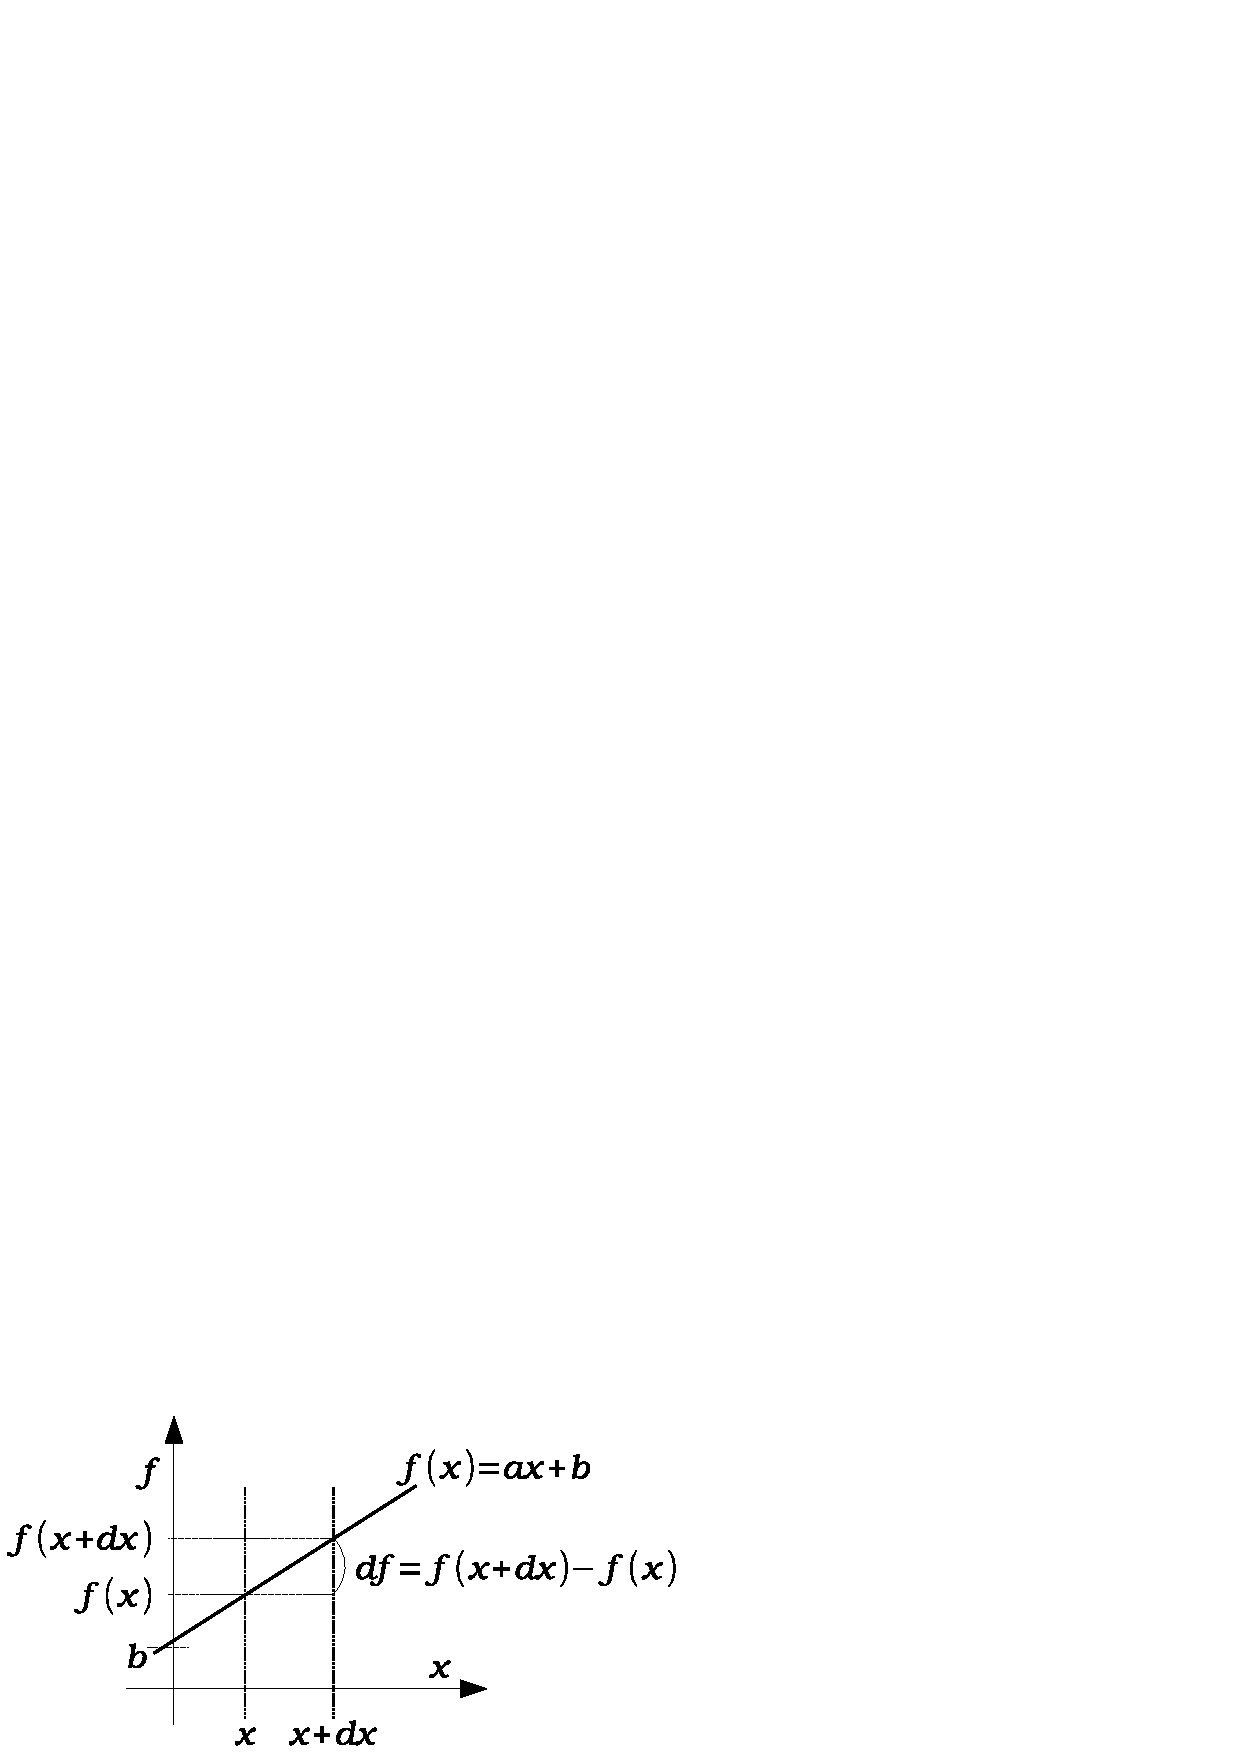
\includegraphics[keepaspectratio, width=6cm,height=2.85cm,clip]{ichi_hensu_kansu_zokaryo2.pdf}
                        \caption{1次関数数関数 $f(x)=ax+b$ の増加量}
                        \label{fig:ichi_hensu_kansu_zokaryo2}
                    \end{center}
                \end{figure}

                一次関数はグラフで表現すると直線であり,
                方程式は $f(x)=ax+b$ である.$a$ は傾きで,$b$ は $y$ 軸との交点である
                        \footnote{
                                $b$ は切片ともよばれる.
                        }.
                                点 $x$ のところでは,
                                        \begin{equation*}
                                                f(x) = ax + b.
                                        \end{equation*}
                                点 $x$ から微小距離 $\df x$ だけ離れたところでは($x+\df x$),
                                        \begin{equation*}
                                                f(x+\df x)=a(x+\df x)+b.
                                        \end{equation*}
                                よって, $x$ が $\df x$ だけ増えた時の $f(x)$ の増加量を $\df f$ として
                                        \footnote{
                                                より細かく表現すると,$\df f := \df f(x)$ である.
                                        },
                                        \begin{align*}
                                                \df f &= f(x+\df x) - f(x) \\
                                                      &= \{a(x+\df x)+b\} - \{ax + b\} \\
                                                      &= (ax + a\df x + b) - (ax + b) \\
                                                      &= a \df x.
                                        \end{align*}

                                一次関数の増加量は傾き $a$ と 微少変化 $\df x$ の積で表せることがわかった.

        %==================================================================
        %  SubSection
        %==================================================================
            \subsection{1変数関数 $f(x)$ の増加量}
                1変数関数 $f(x)$ において,$x$ の微小変化分 $\df x$ に対する $f(x)$ の
                増加量を計算したいことがある.これは,局所的に一次関数近似することで,
                一次関数の時と同じように考えることができる.
                \begin{figure}[hbt]
                    \begin{center}
                        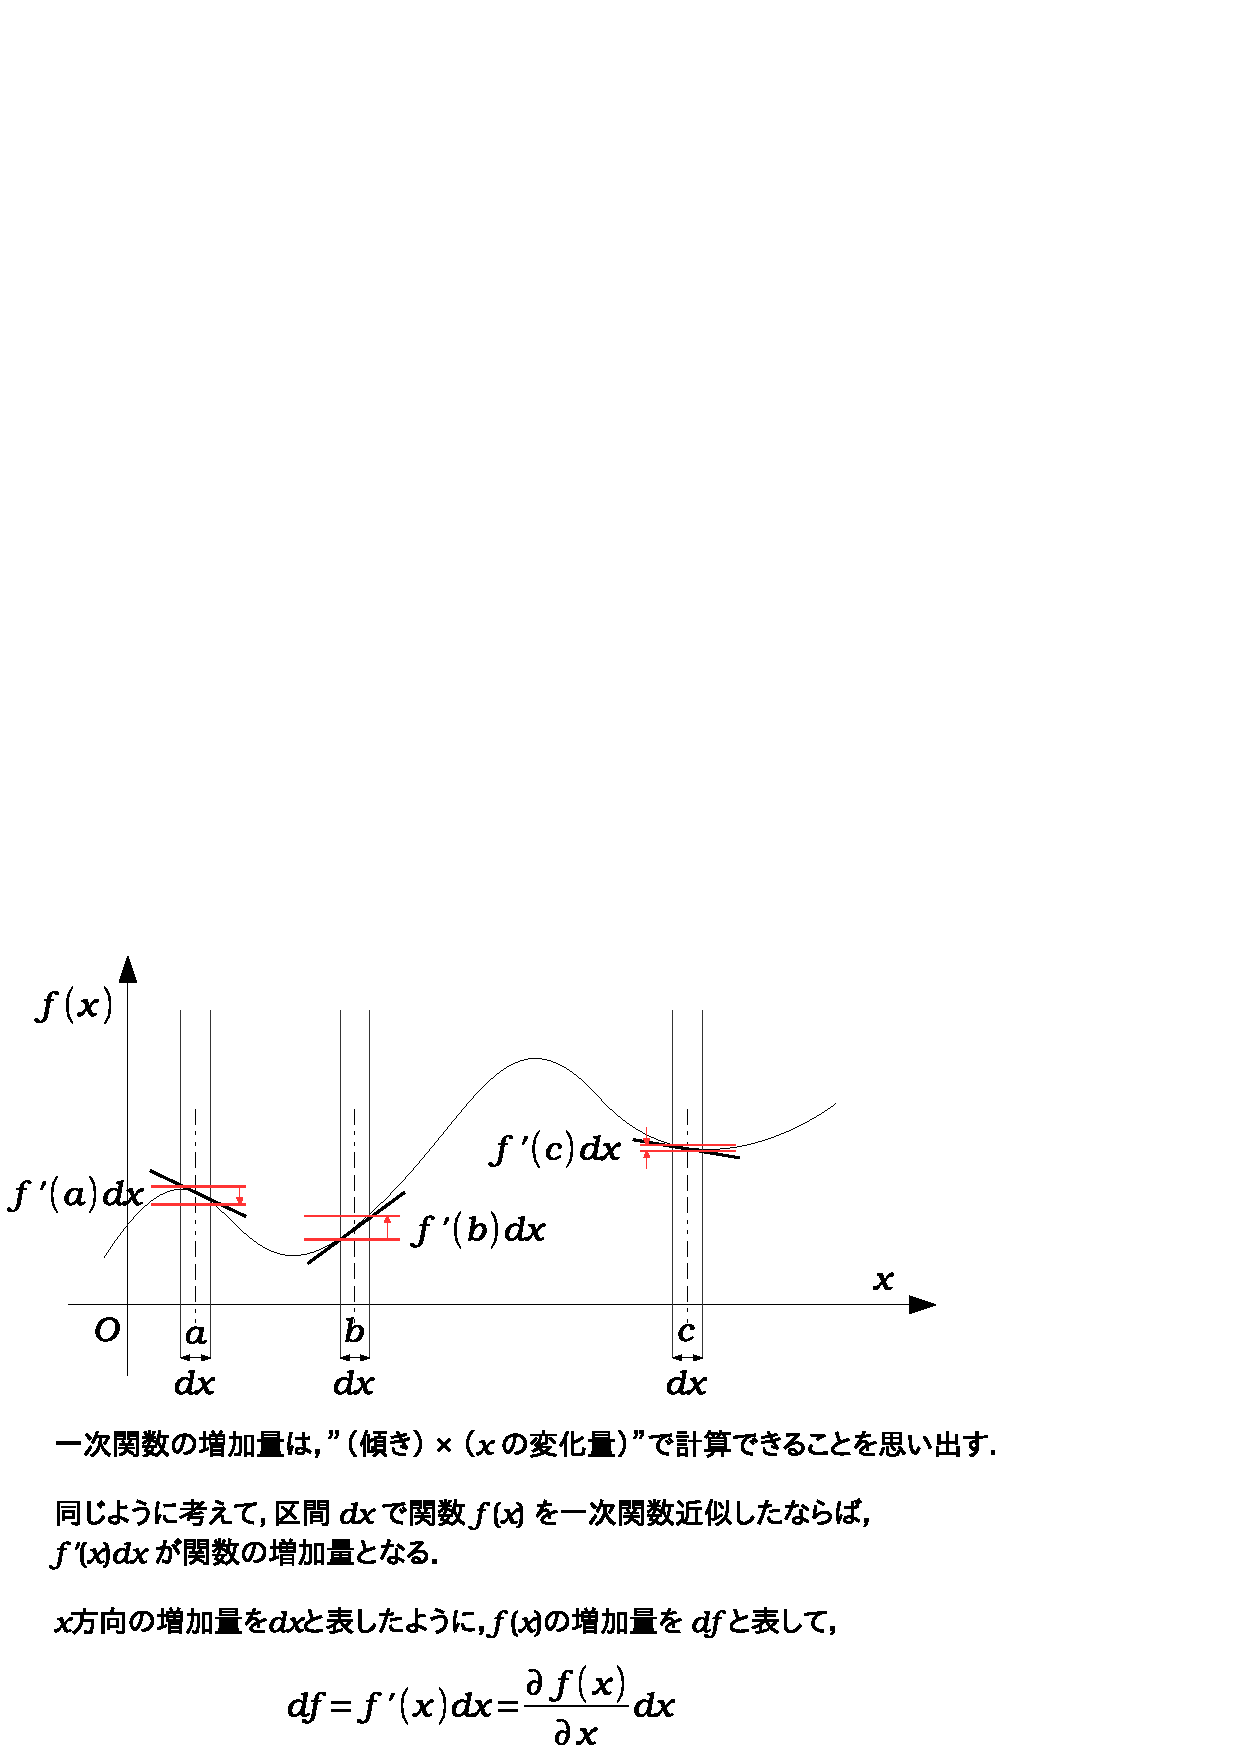
\includegraphics[keepaspectratio, width=7cm,height=6.7cm,clip]{ichi_hensu_kansu_zokaryo1.pdf}
                        \caption{1変数関数 $f(x)$ の増加量}
                        \label{fig:ichi_hensu_kansu_zokaryo1}
                    \end{center}
                \end{figure}

                                一次関数では,微小変化 $\df x$ に対する関数$f$の増加量は,
                                $\df f= a\df x$ と書けるのであった.
                                これを任意の一変数関数に拡張する場合,各$x$ で傾きが異なるが,$a=f'(x)$ と書けることを考慮すると,
                                        \begin{align}
                                                \df f = f'(x) \df x
                                        \end{align}
                                となる.これが1変数関数 $f(x)$ の増加量である.これはまさに,
                                前に説明した \textbf{微分} にほかならない.微分とは一変数関数の微小増加量のことをいうのである.

        %==================================================================
        %  SubSection
        %==================================================================
            \subsection{偏微分}
                次は2変数関数の微分だ.
                1変数関数のグラフは線であり,$x$方向の1方向のみを考えればよかった.
                これに対して,2変数の場合は面になるので,$x$方向と$y$方向の2方向を
                考える必要がある.

                $x$方向の微分をする場合は,$y$方向を固定して微分する.
                式で書くと,
                        \begin{equation*}
                                \frac{\rd f(x,\,y)}{\rd x}
                                := \lim_{\Delta x \to 0} \frac{f(x+\Delta x,\,y)-f(x,\,y)}{\Delta x}.
                        \end{equation*}
                $y$方向の微分をする場合は,$x$方向を固定して微分する.
                式で書くと,
                        \begin{equation*}
                                \frac{\rd f(x,\,y)}{\rd y}
                                := \lim_{\Delta y \to 0} \frac{f(x,\,y+\Delta y)-f(x,\,y)}{\Delta y}.
                        \end{equation*}
                このような微分を1変数の微分と区別するために
                        \footnote{
                                言い換えれば,多変数関数の微分であることを\textbf{強調}するために.
                        },
                \textbf{偏微分} という.

                偏微分の視点で,改めて,1変数の微分を見ると,$y=0$ 固定の微分であったと解釈できる.

        %==================================================================
        %  SubSection
        %==================================================================
            \subsection{全微分}
                偏微分の場合,微分するときに片方を固定してしまうので,$x$ と $y$ を"同時に"変化させた場合
                の関数の増加量がわからない.幸運なことに,$x$ と $y$ を"同時に"変化させた場合の増加量は,
                それぞれ独立であり,
                従って,「$x$ だけを変化させた場合の増加量」と「$y$ だけを変化させた場合の増加量」を
                たすだけで良い.
                \begin{figure}[hbt]
                    \begin{center}
                        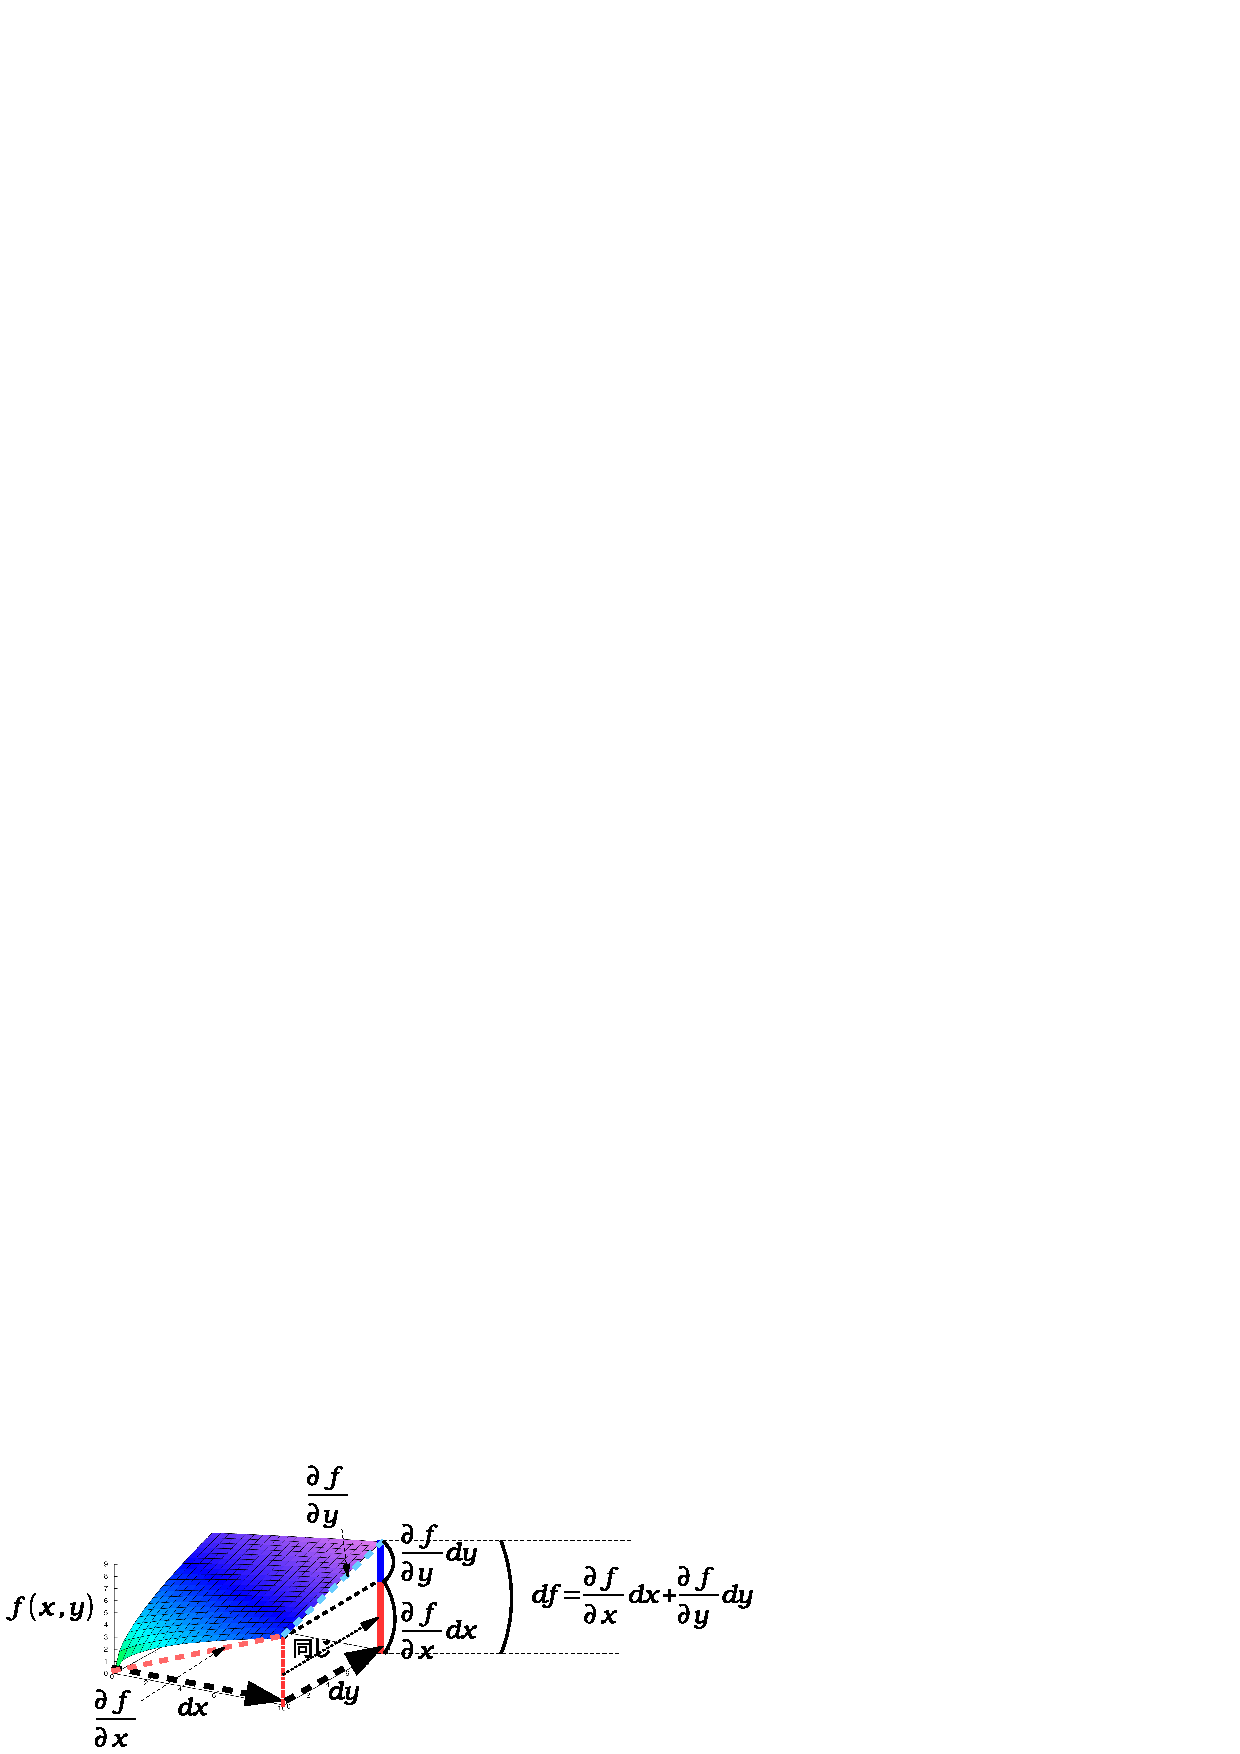
\includegraphics[keepaspectratio, width=7cm,height=4.096cm,clip]{gradient_sample_figure_0001.pdf}
                        \caption{全微分のイメージ}
                        \label{fig:gradient_sample_figure_0001}
                    \end{center}
                \end{figure}

                $x$ 方向だけ変化させた場合の増加量とは,$x$ 方向についての微分であり,
                \begin{equation*}
                     \frac{\rd f(x,\,y)}{\rd x} \df x
               \end{equation*}
                である.また,$y$ 方向だけ変化させた場合の増加量とは,$y$ 方向についての微分であり,
                \begin{equation*}
                    \frac{\rd f(x,\,y)}{\rd y} \df y
                \end{equation*}
                と書ける.よって,$\df f:=\df f(x,\,y)$ は
                \begin{align}
                        \df f = \frac{\rd f(x,\,y)}{\rd x} \df x + \frac{\rd f(x,\,y)}{\rd y} \df y
                \end{align}
                と計算することができる.
                このような2変数関数の微分のことを \textbf{全微分} という.

                もう一度まとめておく.1変数関数の微小増加量が微分であることを先に確認した.
                2変数関数の場合は方向が2つあるので,増加量を計算するには全方向の微分
                \footnote{
                    「全方向の微分」のことを「全独立変数の微分」と言い換えても良い.
                }
                を足し合わせる必要があった.全方向の増加分の和が全微分である.
                2変数以上の関数の微分は全て,全微分と言われる.

                



%   %==========================================================================
%   %  Section : 微分
%   %==========================================================================
        \section{よく使う公式}
%       %----------------------------------------------------------------------
%       %  Input
%       %    File Name : PhysNote_Math_Fomulas.tex
%       %    説明      : よく使われる公式の証明.
%       %----------------------------------------------------------------------
        %       %======================================================================
%       %  SubSection
%       %======================================================================
\subsection{和の微分}
    1変数関数 $K(x)$ があり,この $K(x)$ が2つの関数 $f(x)$,$g(x)$ の和に分解できるとする.
    つまり,以下が成り立っている場合を考える
        \footnote{
            ごく簡単な例で言えば,$K(x)=f(x)+g(x)=5x$,$f(x)=x$,$g(x)=4x$ の場合とか.
        }.
        \begin{equation*}
            K(x) = f(x) + g(x).
        \end{equation*}
    この時,
         \begin{align}
             K'(x) = f'(x) + g'(x)
         \end{align}
    が成り立つ.

    これは微分の定義に従って式変形をすることで,確認できる.少々面倒だが,やってみよう.
        \begin{align*}
            K'(x) &= \lim_{\Delta x \to 0} \frac{K(x+\Delta x)-K(x)}{\Delta x} \\
                  &= \lim_{\Delta x \to 0}
                     \frac{\left(f(x+\Delta x)+g(x+\Delta x)\right)-\left( f(x)+g(x)\right)}{\Delta x} \\
                  &= \lim_{\Delta x \to 0}
                     \frac{f(x+\Delta x)-f(x) + g(x+\Delta x)-g(x)}{\Delta x} \\
                  &= \lim_{\Delta x \to 0}
                     \left(
                         \frac{f(x+\Delta x)-f(x)}{\Delta x}+\frac{g(x+\Delta x)-g(x)}{\Delta x}
                     \right) \\
                  &= \lim_{\Delta x \to 0} \frac{f(x+\Delta x)-f(x)}{\Delta x}
                   + \lim_{\Delta x \to 0} \frac{g(x+\Delta x)-g(x)}{\Delta x} \\
                  &= f'(x) + g'(x).
        \end{align*}

    この式変形で,関数の極限の和の公式を利用している
        \footnote{
            $\displaystyle\lim_{x \to 0}f(x)$ と $\displaystyle\lim_{x \to 0}g(x)$ が共に収束する場合,
            \begin{equation*}
                \lim_{x \to 0}(f(x)+g(x)) = \lim_{x \to 0}f(x) + \lim_{x \to 0}g(x).
            \end{equation*}
        }.

\subsection{積の微分}
    1変数関数 $K(x)$ があり,この $K(x)$ が2つの関数 $f(x)$,$g(x)$ の積に分解できるとする.
    つまり,以下が成り立っている場合を考える
        \footnote{
            ごく簡単な例で言えば,$K(x)=f(x)g(x)=5x(x+1)$,$f(x)=5x$,$g(x)=x+1$ の場合とか.
        }.
        \begin{equation*}
            K(x) = f(x)g(x).
        \end{equation*}
     この時,
         \begin{align}
             K'(x) = f'(x)g(x) + f(x)g'(x)
         \end{align}
     が成り立つ.

    これは微分の定義に従って式変形をすることで,確認できる.少々面倒だが,やってみよう.
    特に,$-f(x)g(x+\Delta x) + f(x)g(x+\Delta x) = 0$ であることに注意.
        \begin{align*}
            &K'(x) \\
            &= \lim_{\Delta x \to 0}
               \frac{K(x+\Delta x)-K(x)}{\Delta x} \\
            &= \lim_{\Delta x \to 0}
               \frac{f(x+\Delta x)g(x+\Delta x)-f(x)g(x)}{\Delta x} \\
            &= \lim_{\Delta x \to 0}
               \frac{f(x+\Delta x)g(x+\Delta x)-f(x)g(x+\Delta x) + f(x)g(x+\Delta x)-f(x)g(x)}{\Delta x} \\
            &= \lim_{\Delta x \to 0}
               \frac{\left(f(x+\Delta x)-f(x)\right)g(x+\Delta x) + f(x)\left(g(x+\Delta x)-g(x)\right)}{\Delta x} \\
            &= \lim_{\Delta x \to 0} \frac{\left(f(x+\Delta x)-f(x)\right)g(x+\Delta x)}{\Delta x}
             + \lim_{\Delta x \to 0} f(x)\frac{g(x+\Delta x)-g(x)}{\Delta x} \\
            &= \lim_{\Delta x \to 0} \frac{f(x+\Delta x)-f(x)}{\Delta x} g(x+\Delta x)
             + f(x) \lim_{\Delta x \to 0} \frac{g(x+\Delta x)-g(x)}{\Delta x} \\
            &= f'(x)g(x) + f(x)g'(x).
        \end{align*}

    この式変形で,関数の極限の積の公式を利用している
        \footnote{
            $\displaystyle\lim_{x \to 0}f(x)$ と $\displaystyle\lim_{x \to 0}g(x)$ が共に収束する場合,
            \begin{equation*}
                \lim_{x \to 0}(f(x) \cdot g(x)) = \lim_{x \to 0}f(x) \cdot \lim_{x \to 0}g(x).
            \end{equation*}
        }.
    また,式変形について,以下を考慮した.
        \begin{align*}
            f(x) &= \lim_{\Delta x \to 0} f(x) \\
            g(x) &= \lim_{\Delta x \to 0} g(x+\Delta x)
        \end{align*}
    1つ目の式はそもそも $\Delta x$ が関数 $f(x)$ にないので,$\Delta x$ に関する極限を
    とったところで変化なし.2つ目の式は関数の極限の定義そのものである.

\subsection{商の微分}
    1変数関数 $K(x)$ があり,この $K(x)$ が2つの関数 $f(x)$,$g(x)$ の商に分解できるとする.
    つまり,以下が成り立っている場合を考える
        \footnote{
            ごく簡単な例で言えば,$K(x)=f(x)/g(x)=5x$,$f(x)=20{x}^{2}$,$g(x)=4x$ の場合とか.
        }.
        \begin{equation*}
            K(x) = \frac{f(x)}{g(x)}.
        \end{equation*}
    この時,
         \begin{align}
             K'(x) = \frac{f'(x)g(x) - f(x)g'(x)}{{\left(g(x)\right)}^{2}}
         \end{align}
    が成り立つ.

    これを示すには,
        \begin{equation*}
            K(x) = \frac{f(x)}{g(x)} = f(x)\frac{1}{g(x)}
        \end{equation*}
    とみなし,積の微分公式を用いる.実際に確認してみよう.
        \begin{equation*}
            K'(x) = f'(x)\frac{1}{g(x)} + f(x)\left(\frac{1}{g(x)}\right)'
        \end{equation*}
    ここで移行の式変形の都合上
        \footnote{
            不自然に思われるかもしれないが,覚えやすく使いやすい形にしたいがための式変形であり,
            重要な部分である.
        }
    ,上式の第1項の分母と分子に $g(x)$ をかけて,
        \begin{equation*}
            K'(x) = f'(x)g(x)\frac{1}{{g(x)}^{2}} + f(x)\left(\frac{1}{g(x)}\right)'
        \end{equation*}
    としておく.また,第2項のカッコ内の微分は,定義に従って計算する
        \footnote{
            2つの分数の恒等式を使うので,補足しておこう.
            \begin{equation*}
                \frac{1}{A} - \frac{1}{B}
                = \frac{B}{AB} - \frac{A}{AB}
                = \frac{B-A}{AB}
                = - \frac{A-B}{AB}.
            \end{equation*}
            \begin{equation*}
                \frac{\displaystyle\frac{A}{B}}{C}
                = \frac{\displaystyle\frac{A}{B}B}{BC}
                = \frac{A}{BC}.
            \end{equation*}
        }.
        \begin{align*}
            \left(\frac{1}{g(x)}\right)'
            &= \lim_{x \to 0}
               \frac{\displaystyle\frac{1}{g(x + \Delta x)} - \displaystyle\frac{1}{g(x)}}{\Delta x} \\
            &= \lim_{x \to 0}
               \frac{\displaystyle\frac{-g(x + \Delta x)+g(x)}{g(x + \Delta x)g(x)}}{\Delta x} \\
            &= \lim_{x \to 0}
               -\frac{g(x + \Delta x)-g(x)}{\Delta x}\frac{1}{{g(x + \Delta x)g(x)}} \\
            &= -g'(x) \frac{1}{{\left(g(x)\right)}^{2}} \\
            &= -\frac{g'(x)}{{\left(g(x)\right)}^{2}}
        \end{align*}
    なので,
        \begin{equation*}
            K'(x) = f'(x)g(x)\frac{1}{{g(x)}^{2}}-f(x)\frac{g'(x)}{{\left(g(x)\right)}^{2}}.
        \end{equation*}
    共通な分母でまとめると,
        \begin{equation*}
            K'(x) = \frac{f'(x)g(x)-f(x)g'(x)}{{\left(g(x)\right)}^{2}}.
        \end{equation*}

\subsection{合成関数の微分}
    関数 $f(g(x))$ というもの考える.$g(x)$ は独立変数 $x$ を持つ関数であり,$f$ は $g(x)$ で
    得られた値を引数に持つ関数である
        \footnote{
            例えば,${(x+1)}^{2}$ であれば,$g(x)=x+1$ として $f(g(x))={\left(g(x)\right)}^{2}$ と
            書き表せる.
        }.
    こういった入れ子になった関数を \textbf{合成関数} という.
    $f(g(x))$ は $(g \circ f)(x)$ と書かれることもある.
        \footnote{
            表記だけの問題だが,$f(g(x))$ という表現は,見難くなる傾向にある.この程度であれば,まだ
            わかるが,これが $f(g(h(i(j(x))))$ となった場合にはカッコが多くて,読み難くくなってしまう.
            だから,$f(g(x))=(g \circ f)(x)$ と書くこともある.これなら,関数が多くなろうとも問題ない.
            さっきの例で言うと,$(j \circ i \circ h \circ g \circ f) (x)$ である.
            関数の依存関係を左のカッコ内に書き,その独立変数を右のカッコの中に書く.関数の依存関係は
            一番深いものを最左に書き,順次右に追記していく.
        }.

    ここでは,この合成関数の微分公式を確認する.
    合成関数 $(g \circ f)(x)=f(g(x))$ は $u=g(x)$ と置いて $f(u)$ と見ることができる.
    $g(x)$ が $x$ の関数だから,結局のところ $(g \circ f)(x)$ も $x$ の関数となるので,
    $\df (g \circ f) /\df x$ を考えられる.$u=g(x)$ を展開し,さらに $f(u)$ を
    展開した後で,微分を計算しても良いが,もっと賢い方法がある.次のとおりだ.
        \begin{align}
            \frac{\df (g \circ f)}{\df x}
            = \frac{\df f}{\df u}\frac{\df u}{\df x}
            = \frac{\df f(u)}{\df u}\frac{\df g(x)}{\df x}.
        \end{align}

    これが正しいことは,微分の定義から計算することで確認できる.
        \begin{align*}
            &\frac{\df (g \circ f)}{\df x} \\
            &= \lim_{\Delta x \to 0}
               \frac{(g \circ f)(x+\Delta x)-(g \circ f)(x)}{\Delta x} \\
            &= \lim_{\Delta x \to 0}
               \frac{(g \circ f)(x+\Delta x)-(g \circ f)(x)}{g(x + \Delta x) - g(x)}
               \frac{g(x + \Delta x) - g(x)}{\Delta x} \\
            &= \lim_{\Delta x \to 0}
               \frac{(g \circ f)(x+\Delta x)-(g \circ f)(x)}{\Delta g}
               \frac{g(x + \Delta x) - g(x)}{\Delta x} \\
            &= \lim_{\Delta x \to 0}
               \frac{(g \circ f)(x+\Delta x)-(g \circ f)(x)}{g(x + \Delta x) - g(x)}
               \cdot
               \lim_{\Delta x \to 0}
               \frac{g(x + \Delta x) - g(x)}{\Delta x}
        \end{align*}

    ここで,式の見やすさのため,$\Delta g = g(x + \Delta x) - g(x)$ と置く.
    また,$g(x)=\displaystyle \lim_{\Delta x \to 0} g(x+\Delta x)$ の関係から,
        \begin{align*}
            &\lim_{\Delta x \to 0} \left( g(x+\Delta x) \right) - g(x) \\
            &= \lim_{\Delta x \to 0} \left( g(x+\Delta x) - g(x) \right) \\
            &= \lim_{\Delta x \to 0} \Delta g \\
            &= 0
        \end{align*} \\
    が成り立つので,$\Delta x \to 0$ を $\Delta g \to 0$ に置き換えられることを使う.
        \begin{flalign*}
            &\frac{\df (g \circ f)}{\df x} \\
                                &= \lim_{\Delta g \to 0}
                                   \frac{(g \circ f)(x+\Delta x)-(g \circ f)(x)}{\Delta g}
                                   \cdot
                                   \lim_{\Delta x \to 0}
                                   \frac{g(x + \Delta x) - g(x)}{\Delta x}
        \end{flalign*}

    最後に,$\Delta (g \circ f) = (g \circ f)(x+\Delta x)-(g \circ f)(x) $,
    $\Delta u = \Delta g$ であることに注意すれば,
        \begin{flalign*}
            \frac{\df (g \circ f)}{\df x}
                &= \lim_{\Delta g \to 0} \frac{\Delta (g \circ f)}{\Delta g}
                   \cdot
                   \lim_{\Delta x \to 0} \frac{g(x + \Delta x) - g(x)}{\Delta x} \\
                &= \lim_{\Delta u \to 0} \frac{\Delta (g \circ f)}{\Delta u}
                   \cdot
                   \lim_{\Delta x \to 0} \frac{\Delta g}{\Delta x} \\
                &= \lim_{\Delta u \to 0} \frac{\Delta (g \circ f)}{\Delta u}
                   \cdot
                   \lim_{\Delta x \to 0} \frac{\Delta u}{\Delta x} \\
                &= \frac{\df (g \circ f)}{\df u} \frac{\df u}{\df x}
        \end{flalign*}
    を得る.大抵の場合は,$f:=(g \circ f)=f(g(x))$ と略記されるので,これに従うと,
        \begin{flalign*}
            \frac{\df f}{\df x} &= \frac{\df f}{\df u} \frac{\df u}{\df x}
        \end{flalign*}
    となって,いつもの合成関数の微分公式が見えてくる.

\subsection{部分積分}



